\documentclass[a4paper,fleqn]{cas-sc}

\usepackage{iftex}
\ifxetex
  \usepackage{fontspec}
  \setmainfont{Liberation Serif}
\else
  \usepackage[utf8]{inputenc}
  \usepackage[T5,T1]{fontenc}
\fi
\usepackage[shorthands=off,vietnamese,english]{babel}
\usepackage{amsmath,amssymb,amsfonts,amsthm}
\usepackage{booktabs}
\usepackage{graphicx}
\usepackage{subcaption}
\usepackage{hyperref}
\usepackage{multirow}
\usepackage{array}
\usepackage{tabularx}
\usepackage{xcolor}
\usepackage{url}

% Định nghĩa các môi trường định lý bằng tiếng Việt
\newtheorem{theorem}{Định lý}
\newtheorem{lemma}{Bổ đề}
\newtheorem{definition}{Định nghĩa}
\newtheorem{proposition}{Mệnh đề}

\begin{document}
\selectlanguage{vietnamese}
\let\WriteBookmarks\relax
\def\floatpagepagefraction{1}
\def\textpagefraction{.001}

% Tiêu đề ngắn và tên tác giả trên tiêu đề trang chạy (running header)
\shorttitle{Nghiên cứu Thực nghiệm SAT Encodings và So sánh Đa Mô hình cho Bài toán N-Queens}
\shortauthors{Trần Nhật Hưng}

% Tiêu đề chính của bài báo
\title [mode = title]{Nghiên cứu Thực nghiệm Chuyên sâu về các Kỹ thuật Mã hóa SAT và So sánh Đa Mô hình (SAT, CP, MIP) cho Bài toán N-Queens}

% Thông tin tác giả
\author[1]{Trần Nhật Hưng}[type=editor,
                        auid=000,bioid=1]
\cormark[1]
\ead{hungthaibinh147@gmail.com}
\address[1]{Khoa Công nghệ Thông tin, Trường Đại học Công nghệ, Đại học Quốc gia Hà Nội, 144 Xuân Thủy, Cầu Giấy, Hà Nội, Việt Nam}

\cortext[cor1]{Tác giả liên hệ chính}

% Tóm tắt bài báo (Abstract)
\begin{abstract}
Bài toán $N$-Queens (Xếp $N$ quân hậu) là một bài toán chuẩn mực (benchmark) kinh điển trong tối ưu hóa tổ hợp, trí tuệ nhân tạo và suy luận tự động, đặt ra yêu cầu sắp đặt $N$ quân hậu trên bàn cờ kích thước $N \times N$ sao cho không có hai quân hậu nào có thể tấn công lẫn nhau. Mặc dù các trường hợp kích thước nhỏ có thể dễ dàng giải quyết bằng thuật toán quay lui (backtracking) cổ điển, việc mở rộng các phương pháp giải chính xác lên quy mô ma trận cực lớn ($N \ge 500$) đặt ra những thách thức bùng nổ tổ hợp to lớn đối với nhiều mô hình tính toán khác nhau. Trong bài báo này, chúng tôi triển khai một nghiên cứu thực nghiệm và lý thuyết chuyên sâu: (1) Đánh giá và phân tích bản chất của năm kỹ thuật mã hóa ràng buộc At-Most-One (AMO) nền tảng trong trường phái Boolean Satisfiability (SAT) Solving---bao gồm Binomial (Pairwise / Cặp đôi), Sequential Counter (Bộ đếm tuần tự), Binary (Mã hóa nhị phân), Commander Variable (Biến chỉ huy với kích thước nhóm $g=3$), và 2-Product; (2) Triển khai thực nghiệm đối đầu đa mô hình (Cross-Paradigm Benchmark) giữa SAT Solving với bốn bộ giải công nghiệp và mã nguồn mở hàng đầu thuộc trường phái Lập trình Ràng buộc (Constraint Programming - CP) và Quy hoạch Tuyến tính Nguyên Hỗn hợp (Mixed Integer Programming - MIP): Google OR-Tools (CP-SAT), IBM ILOG CPLEX CP Optimizer, Gurobi Optimizer (MIP), và IBM ILOG CPLEX MIP.

Không gian thực nghiệm được thiết kế đồng bộ trên chuỗi 15 mốc kích thước từ nhỏ đến quy mô lớn: $N \in [4, 8, 16, 25, 36, 49, 64, 81, 100, 125, 216, 343, 512, 729, 1000]$, đại diện cho mô hình chứa tới $1.000.000$ biến nhị phân và xấp xỉ $14.000.000$ mệnh đề CNF dưới ngưỡng giới hạn thời gian nghiêm ngặt $120.0$ giây mỗi lượt chạy. Kết quả thực nghiệm trên bộ giải Glucose4 (thư viện PySAT) cho thấy mã hóa Binomial gặp phải hiện tượng bùng nổ số lượng mệnh đề bậc bốn ($O(N^4)$), dẫn tới tràn bộ nhớ vật lý (Out-Of-Memory) tại $N \ge 512$ sau khi đã sinh ra hơn $67$ triệu mệnh đề tại $N = 343$. Mặc dù mã hóa Sequential Counter duy trì tính nhất quán cung tổng quát (Generalized Arc Consistency - GAC) qua lan truyền đơn vị (Unit Propagation), lượng biến phụ khổng lồ mà nó tạo ra ($3{,}99 \times 10^6$ biến phụ tại $N = 1000$) làm suy thoái nghiêm trọng hiệu quả của heuristic phân nhánh CDCL, khiến bộ giải bị treo thời gian (timeout) tại $N \ge 343$. Ngược lại, mã hóa Binary thể hiện tính tiết kiệm biến phụ vượt trội ($O(\log m)$), trong khi mã hóa Commander Variable ($g=3$) đạt điểm cân bằng lý tưởng nhất giữa việc giảm số lượng mệnh đề và kiểm soát số lượng biến phụ, giải quyết thành công mốc $N = 1000$ chỉ trong $18{,}92$ giây. 

Trong đối đầu đa mô hình, IBM CPLEX CP Optimizer chứng minh ưu thế thống trị tuyệt đối về tốc độ, giải quyết bài toán kích thước cực đại $N = 1000$ chỉ trong $0{,}250$ giây nhờ thuật toán lan truyền lọc miền giá trị toàn cục của Régin trên ràng buộc $\text{AllDifferent}$. Bên cạnh đó, IBM CPLEX MIP thể hiện độ ổn định phi thường khi giải thành công mốc $N = 1000$ trong $19{,}42$ giây, trong khi Gurobi đạt tốc độ cực nhanh ở miền kích thước trung bình và lớn đến $N = 729$ ($24{,}10$ giây) trước khi chạm ngưỡng timeout. Đáng chú ý, PySAT Glucose4 với mã hóa Commander Variable đã vượt qua cả Gurobi lẫn OR-Tools CP-SAT tại mốc $N = 1000$, khẳng định rằng các bộ giải SAT CDCL hiện đại khi kết hợp cùng kỹ thuật mã hóa ràng buộc tối ưu hoàn toàn đủ năng lực cạnh tranh sòng phẳng hoặc vượt trội so với các bộ giải thương mại đắt giá trên các bài toán thỏa mãn ràng buộc quy mô hàng triệu biến.
\end{abstract}

% Từ khóa (Keywords)
\begin{keywords}
Bài toán N-Queens \sep Mã hóa SAT \sep Ràng buộc At-Most-One (AMO) \sep Thuật toán CDCL \sep Lập trình ràng buộc (CP) \sep Quy hoạch nguyên hỗn hợp (MIP) \sep So sánh đa mô hình \sep PySAT Glucose4
\end{keywords}

\maketitle

% -----------------------------------------------------------------------------
% MỤC 1: GIỚI THIỆU
% -----------------------------------------------------------------------------
\section{Giới thiệu}
\label{sec:intro}

Bài toán $N$-Queens (Xếp $N$ quân hậu) là một trong những bài toán chuẩn mực kinh điển và được nghiên cứu sâu rộng nhất trong lĩnh vực toán học tổ hợp, khoa học máy tính và trí tuệ nhân tạo. Xuất phát điểm từ bài toán 8 quân hậu do kỳ thủ Max Bezzel đề xuất vào năm 1848 \cite{bezzel1848} và được Franz Nauck tổng quát hóa cho kích thước $N$ bất kỳ vào năm 1850 \cite{nauck1850}, mục tiêu của bài toán là tìm cách đặt $N$ quân hậu trên bàn cờ vua kích thước $N \times N$ sao cho không có bất kỳ hai quân hậu nào có thể tấn công lẫn nhau. Theo luật cờ vua, hai quân hậu tấn công nhau nếu chúng cùng nằm trên một hàng, cùng một cột, hoặc cùng một đường chéo (chính hoặc phụ). Như vậy, cấu hình nghiệm đòi hỏi mỗi hàng và mỗi cột phải có đúng một quân hậu, đồng thời mỗi đường chéo trên bàn cờ có không quá một quân hậu.

Vượt ra khỏi phạm vi một trò chơi giải đố thuần túy, bài toán $N$-Queens là bài toán nền tảng để thử nghiệm, đánh giá và kiểm chuẩn các thuật toán tìm kiếm tổ hợp, suy luận tự động và thỏa mãn ràng buộc \cite{bell2009survey,sosic1994polynomial}. Không gian tìm kiếm của bài toán phát triển theo cấp số nhân siêu tốc ($N!$ hoán vị hoặc $N^N$ trạng thái gán tự do), tạo nên thách thức tính toán cực lớn khi kích thước $N$ gia tăng. Bên cạnh đó, các cấu trúc toán học của bài toán $N$-Queens có mối liên hệ trực tiếp với nhiều ứng dụng thực tiễn quan trọng, bao gồm: kiểm thử thiết kế vi mạch tích hợp quy mô rất lớn (VLSI), lập lịch định tuyến bước sóng trong mạng viễn thông cáp quang, phân bổ tài nguyên bộ nhớ song song tránh xung đột truy cập, điều phối đường băng sân bay và bài toán phân rã ma trận thưa \cite{bell2009survey,erbas1992queens}.

Về mặt lịch sử, các phương pháp tiếp cận đầu tiên đối với bài toán $N$-Queens chủ yếu dựa trên thuật toán tìm kiếm quay lui vét cạn (backtracking) và nhánh cận (branch and bound) \cite{golomb1965backtrack,bitner1975backtrack}. Tuy nhiên, các kỹ thuật duyệt cây tìm kiếm truyền thống này gặp phải hiện tượng bùng nổ tổ hợp trầm trọng ngay khi kích thước bàn cờ vượt qua ngưỡng khiêm tốn ($N > 30$). Trong khoa học tính toán hiện đại, ba trường phái giải chính xác khai báo (declarative exact paradigms) đã vươn lên thành các trụ cột giải quyết bài toán thỏa mãn và tối ưu hóa tổ hợp quy mô lớn:
\begin{enumerate}
    \item \textbf{Bộ giải Thỏa mãn Logic Mệnh đề (Boolean Satisfiability - SAT Solving):} Chuyển đổi toàn bộ ràng buộc của bài toán về dạng chuẩn hội (Conjunctive Normal Form - CNF) và giải quyết thông qua các bộ giải SAT hiện đại dựa trên thuật toán Học Mệnh đề theo Xung đột (Conflict-Driven Clause Learning - CDCL). Thuật toán này tích hợp cấu trúc dữ liệu theo dõi hai biến đại diện (Two-Watched Literals - 2WL), heuristic phân nhánh biến dựa trên mức độ hoạt động (VSIDS), và chiến lược quản lý thu dọn mệnh đề học dựa trên khoảng cách khối biến (Literal Block Distance - LBD) \cite{biere2009handbook,audemard2009predicting,moskewicz2001chaff}.
    \item \textbf{Lập trình Ràng buộc (Constraint Programming - CP):} Mô hình hóa bài toán tự nhiên trên các biến nhận giá trị trong miền số nguyên hữu hạn và khai thác sức mạnh của các thuật toán lan truyền lọc miền giá trị toàn cục (global constraint propagators), tiêu biểu nhất là thuật toán lọc ràng buộc $\text{AllDifferent}$ của Régin dựa trên cặp ghép cực đại đồ thị hai phía \cite{regin1994filtering,rossi2006handbook}.
    \item \textbf{Quy hoạch Tuyến tính Nguyên Hỗn hợp (Mixed Integer Programming - MIP / 0-1 ILP):} Thiết lập bài toán dưới dạng hệ phương trình và bất phương trình tuyến tính trên các biến nhị phân 0-1, được giải quyết bằng các mặt cắt đa diện (polyhedral cutting planes), nới lỏng quy hoạch tuyến tính (LP relaxation) và thuật toán nhánh cận đối ngẫu đơn lượng (dual simplex branch-and-cut) \cite{wolsey1999integer,nemhauser1988integer}.
\end{enumerate}

Mặc dù các bộ giải SAT CDCL hiện đại sở hữu tốc độ suy diễn hàng triệu mệnh đề mỗi giây, hiệu năng thực tế của phương pháp SAT phụ thuộc mang tính quyết định vào kỹ thuật mã hóa (encoding) chuyển đổi từ các ràng buộc bậc cao về dạng CNF. Trong bài toán $N$-Queens, điều kiện "mỗi đường chéo, mỗi hàng, mỗi cột có không quá một quân hậu" bản chất là một ràng buộc số lượng \textit{Tối đa một} (At-Most-One - AMO) trên tập hợp $m$ biến logic ($\sum_{i=1}^m x_i \le 1$). Kỹ thuật mã hóa ghép cặp cổ điển \textit{Binomial} (hay Pairwise) cấm trực tiếp từng cặp hai biến đồng thời nhận giá trị True, dẫn tới số lượng mệnh đề bậc hai $\binom{m}{2} = O(m^2)$. Khi áp dụng cho toàn bộ $N$ hàng, $N$ cột và $4N - 2$ đường chéo, tổng số lượng mệnh đề CNF bùng nổ ở bậc bốn $O(N^4)$. Ở quy mô bàn cờ lớn ($N \ge 500$), kỹ thuật này sinh ra hàng trăm triệu mệnh đề, dẫn tới cạn kiệt bộ nhớ RAM (Out-Of-Memory) ngay trong giai đoạn khởi tạo công thức trước khi solver kịp tiến hành tìm kiếm.

Để khắc phục nút thắt cổ chai này, nhiều phương pháp mã hóa SAT nâng cao đã được nghiên cứu và phát triển, sử dụng thêm các biến logic phụ trợ (auxiliary variables) để nén số lượng mệnh đề từ $O(m^2)$ xuống $O(m)$ hoặc $O(m \log m)$ \cite{sinz2005towards,klieber2007commander,chen2010new,frisch2005atmost}. Các kỹ thuật nổi bật gồm: \textit{Sequential Counter} (Bộ đếm tuần tự) \cite{sinz2005towards}, \textit{Binary} (Mã hóa nhị phân) \cite{frisch2005atmost}, \textit{Commander Variable} (Biến chỉ huy) \cite{klieber2007commander}, và \textit{2-Product} \cite{chen2010new}. Tuy nhiên, điều này đặt ra một bài toán đánh đổi cốt lõi trong lý thuyết và thực tiễn: \textit{Liệu việc giảm thiểu số lượng mệnh đề CNF có luôn đồng nghĩa với việc rút ngắn thời gian giải?}

Việc đưa vào quá nhiều biến phụ trợ sẽ mở rộng không gian tìm kiếm Boolean, tiềm ẩn nguy cơ làm sai lệch heuristic định hướng phân nhánh của bộ giải. Mặt khác, các phương pháp mã hóa khác biệt sâu sắc về khả năng bảo toàn tính nhất quán cung tổng quát (Generalized Arc Consistency - GAC) thông qua lan truyền đơn vị (Unit Propagation - UP) \cite{gent2002arc}. Cho đến nay, các công trình so sánh thực nghiệm toàn diện trên cùng một hệ quy chiếu kích thước lớn, vừa đánh giá chi tiết 5 kỹ thuật mã hóa SAT, vừa đặt trong thế đối đầu với các bộ giải CP và MIP công nghiệp hàng đầu thế giới vẫn còn tương đối hạn chế.

\subsection{Các Đóng góp Chính của Bài báo}
Nhằm giải quyết trọn vẹn bài toán trên, công trình này mang lại các đóng góp khoa học chính như sau:
\begin{enumerate}
    \item \textbf{Chuẩn hóa Lý thuyết Toán học Toàn diện:} Thiết lập mô hình toán học giải tích, cấu trúc mệnh đề phân rã và độ phức tạp tiệm cận cho 5 phương pháp mã hóa AMO: Binomial, Sequential Counter, Binary, Commander Variable ($g=3$), và 2-Product.
    \item \textbf{Mô hình hóa Đa Trường phái:} Thiết lập mô hình bài toán $N$-Queens tương ứng trên ba trường phái giải chính xác: Quy hoạch tuyến tính 0-1 (MIP), Lập trình ràng buộc (CP) với ràng buộc toàn cục $\text{AllDifferent}$, và SAT logic mệnh đề.
    \item \textbf{Hệ thống Thực nghiệm Đồng bộ Quy mô Lớn:} Khảo sát toàn diện 5 phương pháp mã hóa SAT và 5 bộ giải độc lập---PySAT Glucose4, Google OR-Tools CP-SAT, IBM ILOG CPLEX CP Optimizer, Gurobi Optimizer (MIP), và IBM ILOG CPLEX MIP---trên chuỗi 15 mốc kích thước đồng bộ:
    \[
    N \in \{4, 8, 16, 25, 36, 49, 64, 81, 100, 125, 216, 343, 512, 729, 1000\}.
    \]
    Mốc kích thước cực đại $N = 1000$ (tương ứng $1.000.000$ biến nhị phân) được giải quyết với bản quyền học thuật đầy đủ, cung cấp số liệu thực nghiệm chính xác cao.
    \item \textbf{Phát hiện và Lý giải các Hiện tượng Thực nghiệm Sâu sắc:}
    \begin{itemize}
        \item *Bức tường Bộ nhớ Binomial:* Lý giải nguyên nhân khiến Binomial cạn kiệt bộ nhớ tại $N \ge 512$.
        \item *Nghịch lý Bộ đếm Tuần tự (Sequential Counter):* Phân tích lý do vì sao một kỹ thuật bảo toàn GAC lý thuyết lại thất bại và timeout ở $N \ge 343$ do sự bùng nổ của $3{,}99 \times 10^6$ biến phụ trợ làm "nhiễu loạn" heuristic VSIDS.
        \item *Hiệu quả Đột phá của Binary và Commander:* Chứng minh khả năng nén biến phụ vượt bậc của Binary ($O(\log m)$) và sự cân bằng tuyệt hảo của Commander Variable ($g=3$), giúp Glucose4 giải $N = 1000$ trong $18{,}92$ giây.
        \item *Sức mạnh Vô địch của Lọc Miền Giá trị Toàn cục CP:* Phân tích nguyên nhân giúp IBM CPLEX CP giải quyết bàn cờ $N = 1000$ trong vỏn vẹn $0{,}250$ giây nhờ thuật toán cặp ghép cực đại của Régin.
    \end{itemize}
    \item \textbf{Tính Sẵn sàng và Tái lập Dữ liệu (Open Science):} Toàn bộ mã nguồn, các script benchmark tự động, dữ liệu thực nghiệm thô dạng CSV và các Jupyter Notebook trực quan hóa đã được công khai trên GitHub Repository \cite{hung2026github}.
\end{enumerate}

\subsection{Cấu trúc Bài báo}
Phần còn lại của bài báo được tổ chức như sau: Mục~\ref{sec:background} trình bày định nghĩa hình thức bài toán $N$-Queens, cùng các mô hình MIP, CP và nguyên lý hoạt động của bộ giải SAT CDCL. Mục~\ref{sec:sat_encodings} đi sâu vào bản chất toán học, công thức sinh mệnh đề và độ phức tạp của năm kỹ thuật mã hóa AMO. Mục~\ref{sec:experiments} trình bày chi tiết thiết lập thực nghiệm, phân tích kết quả so sánh giữa các mã hóa SAT, kết quả đối đầu đa mô hình, cùng thảo luận chuyên sâu về các hiện tượng thực nghiệm và bảng ma trận khuyến nghị. Cuối cùng, Mục~\ref{sec:conclusion} tổng kết bài báo và mở ra các định hướng nghiên cứu tiếp theo.

% -----------------------------------------------------------------------------
% MỤC 2: CƠ SỞ LÝ THUYẾT VÀ MÔ HÌNH HÓA BÀI TOÁN
% -----------------------------------------------------------------------------
\section{Cơ sở Lý thuyết và Mô hình Hóa Bài toán}
\label{sec:background}

\subsection{Định nghĩa Toán học Bài toán N-Queens}
Cho $\mathcal{B}_N = \{0, 1, \dots, N-1\} \times \{0, 1, \dots, N-1\}$ biểu diễn bàn cờ vuông kích thước $N \times N$, trong đó mỗi ô cờ được xác định bởi cặp tọa độ $(i, j)$ tương ứng với hàng $i$ và cột $j$. Bài toán $N$-Queens yêu cầu xác định vị trí đặt của đúng $N$ quân hậu trên bàn cờ $\mathcal{B}_N$ sao cho không có bất kỳ hai quân hậu nào có thể khống chế lẫn nhau.

Theo quy tắc cờ vua tiêu chuẩn, quân hậu tại ô $(i, j)$ sẽ kiểm soát tất cả các ô nằm trên:
\begin{enumerate}
    \item Cùng hàng $i$: các ô $(i, j')$ với $j' \neq j$;
    \item Cùng cột $j$: các ô $(i', j)$ với $i' \neq i$;
    \item Cùng đường chéo chính: các ô $(i', j')$ thỏa mãn hiệu chỉ số bằng nhau: $i' - j' = i - j$;
    \item Cùng đường chéo phụ: các ô $(i', j')$ thỏa mãn tổng chỉ số bằng nhau: $i' + j' = i + j$.
\end{enumerate}

Cấu hình nghiệm hợp lệ của bài toán được hình thức hóa thông qua định nghĩa toán học sau:
\begin{definition}[Nghiệm hợp lệ của Bài toán $N$-Queens]
Một cách đặt $N$ quân hậu trên bàn cờ $\mathcal{B}_N$ là nghiệm hợp lệ khi và chỉ khi thỏa mãn đồng thời bốn điều kiện sau:
\begin{align}
    &\text{Mỗi hàng có đúng một quân hậu;} \label{eq:cond_row}\\
    &\text{Mỗi cột có đúng một quân hậu;} \label{eq:cond_col}\\
    &\text{Mỗi đường chéo chính có tối đa một quân hậu;} \label{eq:cond_diag}\\
    &\text{Mỗi đường chéo phụ có tối đa một quân hậu.} \label{eq:cond_antidiag}
\end{align}
\end{definition}

Vì bàn cờ có $N$ hàng và cần đặt $N$ quân hậu, điều kiện (\ref{eq:cond_row}) tự động đảm bảo rằng không thể có hai quân hậu nào cùng hàng. Tương tự, điều kiện (\ref{eq:cond_col}) ngăn chặn việc hai quân hậu cùng cột. Bàn cờ chứa tổng cộng $2N - 1$ đường chéo chính (được chỉ số hóa bởi $k = i - j \in \{-(N-1), \dots, N-1\}$) và $2N - 1$ đường chéo phụ ($k = i + j \in \{0, \dots, 2N-2\}$). Các đường chéo chỉ chứa một ô duy nhất tại góc bàn cờ (ví dụ $i - j = N-1$ hoặc $i + j = 0$) luôn tự động thỏa mãn điều kiện tối đa một quân hậu; do đó, các ràng buộc đường chéo chỉ cần áp dụng cho các đường có độ dài $\ge 2$.

\subsection{Mô hình Quy hoạch Tuyến tính Nguyên Hỗn hợp (0-1 MIP)}
Trong mô hình Quy hoạch Tuyến tính Nguyên 0-1 (MIP / ILP), trạng thái bàn cờ được biểu diễn thông qua ma trận các biến quyết định nhị phân:
\begin{equation}
    x_{i,j} \in \{0, 1\}, \quad \forall i, j \in \{0, 1, \dots, N-1\},
\end{equation}
trong đó $x_{i,j} = 1$ biểu thị có một quân hậu được đặt tại ô $(i, j)$, và $x_{i,j} = 0$ nếu ô đó trống.

Hệ thống các ràng buộc tuyến tính của bài toán được thiết lập như sau:
\begin{align}
    &\sum_{j=0}^{N-1} x_{i,j} = 1, \quad \forall i \in \{0, \dots, N-1\} \quad \text{(Ràng buộc Hàng)}, \label{eq:mip_row}\\
    &\sum_{i=0}^{N-1} x_{i,j} = 1, \quad \forall j \in \{0, \dots, N-1\} \quad \text{(Ràng buộc Cột)}, \label{eq:mip_col}\\
    &\sum_{\substack{0 \le i, j < N \\ i - j = k}} x_{i,j} \le 1, \quad \forall k \in \{-(N-2), \dots, N-2\} \quad \text{(Đường chéo chính)}, \label{eq:mip_diag}\\
    &\sum_{\substack{0 \le i, j < N \\ i + j = k}} x_{i,j} \le 1, \quad \forall k \in \{1, \dots, 2N-3\} \quad \text{(Đường chéo phụ)}. \label{eq:mip_antidiag}
\end{align}

\begin{proposition}[Quy mô Mô hình 0-1 MIP]
Mô hình quy hoạch nguyên 0-1 chuẩn của bài toán $N$-Queens bao gồm đúng $N^2$ biến nhị phân và $6N - 6$ ràng buộc tuyến tính (gồm $N$ đẳng thức hàng, $N$ đẳng thức cột, $2N - 3$ bất đẳng thức đường chéo chính và $2N - 3$ bất đẳng thức đường chéo phụ).
\end{proposition}

\subsubsection{Đặc tính Đa diện và Nới lỏng Tuyến tính (LP Relaxation)}
Trong lý thuyết đa diện tổ hợp, bài toán $N$-Queens có một đặc điểm nổi tiếng: bài toán nới lỏng tuyến tính liên tục (LP Relaxation, khi thay $x_{i,j} \in \{0, 1\}$ bằng $x_{i,j} \in [0, 1]$) có tính chất cực kỳ yếu \cite{wolsey1999integer}. Cụ thể, nghiệm phân số đồng nhất $x_{i,j} = \frac{1}{N}$ với mọi $i, j$ luôn thỏa mãn toàn bộ các ràng buộc đẳng thức hàng, cột và bất đẳng thức đường chéo ($\sum \frac{1}{N} \le \frac{N-|k|}{N} \le 1$). 

Do đó, hàm mục tiêu nới lỏng không cung cấp bất kỳ thông tin dẫn đường nào cho thuật toán nhánh cận thông thường nếu chỉ dựa vào đơn hình đối ngẫu thuần túy. Các bộ giải MIP thương mại hàng đầu như Gurobi và IBM CPLEX MIP giải quyết được bài toán này ở quy mô lớn là nhờ vào các thuật toán tiền xử lý (presolve) tinh vi, suy luận dựa trên đồ thị xung đột (conflict graphs), sinh mặt cắt clique cuts, và các heuristic tìm kiếm nghiệm nguyên khả thi tiên tiến \cite{bixby2002solving,achterberg2013gurobi}.

\subsection{Mô hình Lập trình Ràng buộc (Constraint Programming - CP)}
Trường phái Lập trình Ràng buộc (CP) biểu diễn bài toán thông qua các biến miền nguyên và các ràng buộc toàn cục (global constraints) mang tính biểu đạt cao \cite{rossi2006handbook}. Thay vì sử dụng ma trận $N^2$ biến nhị phân, bài toán $N$-Queens được mô hình hóa tinh gọn bằng một vector gồm đúng $N$ biến nguyên:
\begin{equation}
    q_i \in \{0, 1, \dots, N-1\}, \quad \forall i \in \{0, 1, \dots, N-1\},
\end{equation}
trong đó giá trị của $q_i$ đại diện trực tiếp cho chỉ số cột của quân hậu nằm tại hàng thứ $i$.

Nhờ cách thiết kế này, điều kiện (\ref{eq:cond_row}) (mỗi hàng đúng một quân hậu) được tự động thỏa mãn mà không cần bất kỳ ràng buộc nào, bởi mỗi biến $q_i$ tương ứng duy nhất với hàng $i$ và chỉ nhận một giá trị duy nhất. Việc loại trừ xung đột cột và hai hướng đường chéo được mô hình hóa hoàn hảo thông qua đúng ba ràng buộc toàn cục $\text{AllDifferent}$:
\begin{align}
    &\text{AllDifferent}\big(q_0, q_1, \dots, q_{N-1}\big) \quad \text{(Không cùng cột)}, \label{eq:cp_col}\\
    &\text{AllDifferent}\big(q_0 - 0, q_1 - 1, \dots, q_{N-1} - (N-1)\big) \quad \text{(Không cùng chéo chính)}, \label{eq:cp_diag}\\
    &\text{AllDifferent}\big(q_0 + 0, q_1 + 1, \dots, q_{N-1} + (N-1)\big) \quad \text{(Không cùng chéo phụ)}. \label{eq:cp_antidiag}
\end{align}

\subsubsection{Thuật toán Lọc Miền Giá trị Toàn cục của Régin}
Sức mạnh vượt trội của mô hình CP nằm ở bộ lọc lan truyền gắn liền với ràng buộc $\text{AllDifferent}$. Nếu phân rã ràng buộc này thành $\binom{N}{2}$ cặp bất đẳng thức cơ bản ($q_i \neq q_j$), bộ giải chỉ đạt được tính nhất quán cặp (pairwise consistency) rất yếu. Năm 1994, Jean-Charles Régin đã công bố thuật toán lọc mang tính bước ngoặt \cite{regin1994filtering}, cho phép duy trì tính nhất quán cung tổng quát (GAC) trên toàn bộ ràng buộc $\text{AllDifferent}$ trong thời gian đa thức.

Thuật toán Régin ánh xạ bài toán sang đồ thị hai phía $G = (X \cup Y, E)$, với $X = \{q_0, \dots, q_{N-1}\}$ là tập đỉnh biến, $Y = \{0, \dots, N-1\}$ là tập đỉnh giá trị, và cạnh $(q_i, v) \in E$ tồn tại khi giá trị $v$ thuộc miền xác định hiện thời $\text{dom}(q_i)$. Một phép gán hợp lệ tương ứng với một cặp ghép cực đại phủ toàn bộ $X$, được tìm kiếm thông qua thuật toán Hopcroft--Karp trong thời gian $O(N^{1.5} \cdot |E|)$. Bằng cách định chiều đồ thị và phân tích các thành phần liên thông mạnh (SCC) thông qua thuật toán Tarjan, bộ lọc của Régin xác định chính xác và loại bỏ triệt để tất cả các cạnh không bao giờ có thể thuộc về bất kỳ cặp ghép cực đại nào. Nhờ sự thu hẹp miền giá trị thần tốc này, không gian tìm kiếm bị thu hẹp đáng kể, giúp bộ giải CP tìm ra nghiệm gần như tức thì mà không bị quay lui.

\subsection{Logic Mệnh đề, Dạng Chuẩn Hội (CNF) và Bộ giải SAT CDCL}
Bài toán Thỏa mãn Logic Mệnh đề (Boolean Satisfiability - SAT) kiểm tra xem liệu có tồn tại một phép gán chân trị (True/False) cho các biến logic sao cho công thức mệnh đề nhận giá trị True hay không. Một công thức $\mathcal{F}$ biểu diễn dưới Dạng Chuẩn Hội (Conjunctive Normal Form - CNF) là một phép hội của các mệnh đề (clauses):
\begin{equation}
    \mathcal{F} = \bigwedge_{c=1}^C \mathcal{C}_c, \quad \text{trong đó } \mathcal{C}_c = \bigvee_{l \in \mathcal{C}_c} l,
\end{equation}
và mỗi literal $l$ là một biến $v$ hoặc phủ định của nó $\neg v$.

Các bộ giải SAT hiện đại hoạt động dựa trên cấu trúc giải thuật CDCL (Conflict-Driven Clause Learning) \cite{biere2009handbook}, bao gồm các thành phần cốt lõi:
\begin{itemize}
    \item \textbf{Lan truyền Đơn vị (Unit Propagation - UP) và Two-Watched Literals (2WL):} Khi một mệnh đề chỉ còn đúng một literal chưa gán chân trị và tất cả các literal còn lại đều đã mang giá trị False, literal duy nhất đó bắt buộc phải được gán True. Cơ chế 2WL \cite{moskewicz2001chaff} chỉ theo dõi hai literal chưa False trong mỗi mệnh đề, giúp bộ giải bỏ qua phần lớn các mệnh đề trong quá trình gán giá trị, đạt tốc độ hàng triệu phép thử mỗi giây.
    \item \textbf{Phân tích Xung đột và Học Mệnh đề (Clause Learning):} Khi xảy ra xung đột (một mệnh đề có tất cả literal mang giá trị False), bộ giải duyệt ngược đồ thị suy diễn để xác định Điểm Hàm ý Duy nhất Thứ nhất (First Unique Implication Point - 1UIP), sinh ra một mệnh đề học mới và bổ sung vào cơ sở dữ liệu, ngăn solver lặp lại sai lầm trong tương lai.
    \item \textbf{Quay lui Phi Tuần tự (Backjumping):} Thay vì lùi từng bước như DFS, bộ giải nhảy ngược thẳng về mức quyết định thấp nhất do mệnh đề học quy định.
    \item \textbf{Heuristic Đo lường Chất lượng Mệnh đề LBD (Literal Block Distance):} Được phát triển bởi Audemard và Simon trong bộ giải Glucose \cite{audemard2009predicting}, LBD đếm số lượng mức quyết định khác nhau xuất hiện trong mệnh đề học. Các mệnh đề có chỉ số LBD nhỏ được xem là các mệnh đề "keo" (glue clauses) có chất lượng cao nhất và được ưu tiên lưu giữ vĩnh viễn trong bộ nhớ.
\end{itemize}

% -----------------------------------------------------------------------------
% MỤC 3: CÁC KỸ THUẬT MÃ HÓA SAT CHO BÀI TOÁN N-QUEENS
% -----------------------------------------------------------------------------
\section{Các Kỹ thuật Mã hóa SAT cho Bài toán N-Queens}
\label{sec:sat_encodings}

\subsection{Phân rã Ràng buộc Bàn cờ}
Để mô hình hóa bài toán $N$-Queens sang CNF, chúng ta định nghĩa $N^2$ biến quyết định Boolean ban đầu:
\begin{equation}
    x_{i,j} \in \{\text{True}, \text{False}\}, \quad \forall i, j \in \{0, 1, \dots, N-1\},
\end{equation}
trong đó $x_{i,j} = \text{True}$ khi và chỉ khi có một quân hậu ngự trị tại ô $(i, j)$ của bàn cờ.

Mỗi nhóm ô cờ cần quản lý $X = \{u_1, u_2, \dots, u_m\}$ sẽ chịu sự chi phối của một trong hai dạng ràng buộc số lượng:
\begin{enumerate}
    \item \textbf{Đúng một (Exactly-One - EO):} Có đúng một biến trong $X$ nhận giá trị True (cho từng hàng và từng cột).
    \item \textbf{Tối đa một (At-Most-One - AMO):} Có không quá một biến trong $X$ nhận giá trị True (cho từng đường chéo chính và đường chéo phụ).
\end{enumerate}

Ràng buộc Exactly-One được phân rã thành phép hội của ràng buộc \textit{Ít nhất một} (At-Least-One - ALO) và ràng buộc \textit{Tối đa một} (At-Most-One - AMO):
\begin{equation}
    \text{EO}(X) = \text{ALO}(X) \land \text{AMO}(X).
\end{equation}

Ràng buộc ALO được biểu diễn đơn giản qua đúng một mệnh đề tuyển duy nhất có độ dài $m$:
\begin{equation}
    \text{ALO}(X) = \bigvee_{i=1}^m u_i = (u_1 \lor u_2 \lor \dots \lor u_m).
\end{equation}

Đối với toàn bộ bàn cờ $N \times N$, việc thiết lập ALO cho $N$ hàng và $N$ cột chỉ tiêu tốn đúng $2N$ mệnh đề. Toàn bộ độ phức tạp và sự khác biệt về hiệu năng giải SAT tập trung hoàn toàn vào kỹ thuật mã hóa các ràng buộc At-Most-One (AMO). Dưới đây, chúng tôi trình bày chi tiết năm phương pháp mã hóa AMO được khảo sát trong nghiên cứu này.

\subsection{Năm Phương pháp Mã hóa At-Most-One (AMO)}

\subsubsection{Mã hóa Binomial (Pairwise / Cặp đôi)}
Mã hóa Binomial là phương pháp tự nhiên và trực tiếp nhất. Phương pháp này cấm rõ ràng từng cặp hai biến bất kỳ trong $X$ cùng đồng thời nhận giá trị True:
\begin{equation}
    \text{AMO}_{\text{pair}}(X) = \bigwedge_{1 \le i < j \le m} (\neg u_i \lor \neg u_j).
\end{equation}

\begin{proposition}[Độ phức tạp Mã hóa Binomial]
Đối với tập hợp gồm $m$ biến, mã hóa Binomial sinh ra:
\begin{itemize}
    \item Biến phụ trợ: $0$.
    \item Số mệnh đề: $\binom{m}{2} = \frac{m(m-1)}{2} = O(m^2)$.
\end{itemize}
Đối với toàn bộ bài toán $N$-Queens, tổng số lượng mệnh đề CNF do mã hóa Binomial sinh ra có bậc tiệm cận là:
\begin{equation}
    C_{\text{binomial}}(N) = 2N \cdot \binom{N}{2} + 2 \sum_{k=2}^{N-1} 2\binom{k}{2} + 2\binom{N}{2} + 2N = O(N^4).
\end{equation}
\end{proposition}

\textit{Đặc tính lý thuyết:} Mã hóa Binomial duy trì tính nhất quán cung tổng quát (GAC) thông qua lan truyền đơn vị (UP): ngay khi một biến $u_i = \text{True}$, tất cả các mệnh đề $(\neg u_i \lor \neg u_j)$ lập tức trở thành mệnh đề đơn vị và suy diễn $\neg u_j = \text{False}$ với mọi $j \neq i$. Tuy nhiên, tốc độ tăng trưởng bậc bốn $O(N^4)$ khiến bộ nhớ bị tràn khi kích thước $N$ đạt ngưỡng vài trăm.

\subsubsection{Mã hóa Bộ đếm Tuần tự (Sequential Counter)}
Được Carsten Sinz đề xuất vào năm 2005 \cite{sinz2005towards}, mã hóa Bộ đếm Tuần tự thiết lập một chuỗi thanh ghi tích lũy gồm $m - 1$ biến phụ trợ Boolean:
\begin{equation}
    S = \{s_1, s_2, \dots, s_{m-1}\},
\end{equation}
trong đó biến $s_i = \text{True}$ mang ngữ nghĩa: có ít nhất một biến trong đoạn tiền tố $\{u_1, u_2, \dots, u_i\}$ nhận giá trị True.

Ràng buộc AMO được định nghĩa thông qua hệ thống các mệnh đề:
\begin{enumerate}
    \item \textbf{Khởi tạo biến đầu tiên:}
    \begin{equation}
        (\neg u_1 \lor s_1).
    \end{equation}
    \item \textbf{Bước chuyển tiếp tích lũy} ($1 < i < m$):
    \begin{align}
        &(\neg s_{i-1} \lor s_i) \quad \text{(Lan truyền thanh ghi)},\\
        &(\neg u_i \lor s_i) \quad \text{(Kích hoạt thanh ghi khi biến True)},\\
        &(\neg u_i \lor \neg s_{i-1}) \quad \text{(Cấm biến True nếu tiền tố đã True)}.
    \end{align}
    \item \textbf{Mệnh đề chốt chặn phần tử cuối cùng:}
    \begin{equation}
        (\neg u_m \lor \neg s_{m-1}).
    \end{equation}
\end{enumerate}

\begin{proposition}[Độ phức tạp Bộ đếm Tuần tự]
Với ràng buộc có $m$ biến, mã hóa Sequential Counter cần:
\begin{itemize}
    \item Biến phụ trợ: $m - 1 = O(m)$.
    \item Số mệnh đề: $1 + 3(m - 2) + 1 = 3m - 4 = O(m)$.
\end{itemize}
Đối với toàn bộ bài toán $N$-Queens, tổng số lượng mệnh đề giảm ngoạn mục từ $O(N^4)$ xuống còn $O(N^2)$.
\end{proposition}

\textit{Đặc tính lý thuyết:} Phương pháp này bảo toàn đầy đủ tính nhất quán cung tổng quát (GAC) qua lan truyền đơn vị \cite{sinz2005towards}. Tuy nhiên, việc bổ sung $O(N^2)$ biến phụ trợ vào không gian tìm kiếm sẽ tạo ra gánh nặng phân nhánh cực lớn cho bộ giải CDCL như sẽ được phân tích ở Mục~\ref{sec:experiments}.

\subsubsection{Mã hóa Nhị phân (Binary / Bitwise)}
Mã hóa Nhị phân \cite{frisch2005atmost} sử dụng hệ thống số nhị phân để mã hóa sự xung đột chỉ với một lượng biến phụ trợ tỉ lệ logarit. Đặt $k = \lceil \log_2 m \rceil$. Chúng ta cấp phát $k$ biến phụ trợ đại diện cho các bit:
\begin{equation}
    Y = \{y_0, y_1, \dots, y_{k-1}\}.
\end{equation}

Mỗi chỉ số biến $i \in \{0, 1, \dots, m-1\}$ được biểu diễn bằng chuỗi nhị phân $k$-bit duy nhất $\text{bin}(i) = (b_{i,0}, b_{i,1}, \dots, b_{i,k-1})$ với $b_{i,j} \in \{0, 1\}$. Ràng buộc quy định rằng nếu biến $u_i$ nhận giá trị True, trạng thái của các biến bit $Y$ bắt buộc phải trùng khớp với mã nhị phân của $i$:
\begin{equation}
    \text{AMO}_{\text{binary}}(X) = \bigwedge_{i=0}^{m-1} \bigwedge_{j=0}^{k-1} \Big(\neg u_i \lor \phi(i, j)\Big),
\end{equation}
trong đó literal $\phi(i, j)$ được gán:
\begin{equation}
    \phi(i, j) = \begin{cases}
        y_j & \text{nếu } b_{i,j} = 1, \\
        \neg y_j & \text{nếu } b_{i,j} = 0.
    \end{cases}
\end{equation}

Nếu có hai biến khác nhau $u_p$ và $u_q$ ($p \neq q$) cùng nhận True, các biến $Y$ buộc phải đồng thời mang giá trị nhị phân của $p$ và $q$. Vì $p \neq q$, chắc chắn tồn tại ít nhất một vị trí bit $j$ sao cho $b_{p,j} \neq b_{q,j}$, dẫn tới việc biến $y_j$ vừa phải nhận True vừa phải nhận False, lập tức tạo ra xung đột $(y_j \land \neg y_j)$.

\begin{proposition}[Độ phức tạp Mã hóa Nhị phân]
Với ràng buộc độ dài $m$, mã hóa Binary sinh ra:
\begin{itemize}
    \item Biến phụ trợ: $\lceil \log_2 m \rceil = O(\log m)$.
    \item Số mệnh đề: $m \lceil \log_2 m \rceil = O(m \log m)$.
\end{itemize}
Đối với toàn bộ bài toán $N$-Queens, tổng số lượng mệnh đề có bậc $O(N^2 \log N)$, nhưng tổng số lượng biến phụ trợ chỉ tăng ở mức $O(N \log N)$.
\end{proposition}

\textit{Đặc tính lý thuyết:} Mã hóa Binary không duy trì GAC qua lan truyền đơn vị \cite{frisch2005atmost}. Tuy nhiên, nhờ lượng biến phụ trợ cực kỳ khiêm tốn, nó kiểm soát tối đa kích thước của cây phân nhánh CDCL.

\subsubsection{Mã hóa Biến Chỉ huy (Commander Variable)}
Được đề xuất bởi Klieber và Kwon (2007) \cite{klieber2007commander}, mã hóa Commander Variable chia tập biến ban đầu $X$ thành các nhóm nhỏ rời nhau có kích thước cố định $g$ (thường chọn $g=3$):
\begin{equation}
    X = G_1 \cup G_2 \cup \dots \cup G_{\lceil m/g \rceil}, \quad |G_k| \le g.
\end{equation}

Mỗi nhóm $G_k$ được chỉ định một \textit{biến chỉ huy} phụ trợ $c_k$, đại diện cho việc có biến nào trong nhóm $G_k$ nhận True hay không. Ràng buộc gồm 4 điều kiện:
\begin{enumerate}
    \item \textbf{Cấm cặp trong nội bộ nhóm:} Tối đa một biến trong $G_k$ nhận True:
    \begin{equation}
        \bigwedge_{u, v \in G_k, u \neq v} (\neg u \lor \neg v).
    \end{equation}
    \item \textbf{Kích hoạt chỉ huy:} Nếu có biến trong $G_k$ nhận True thì $c_k$ bắt buộc phải True:
    \begin{equation}
        \bigwedge_{u \in G_k} (\neg u \lor c_k).
    \end{equation}
    \item \textbf{Cam kết chỉ huy:} Nếu $c_k$ nhận True thì ít nhất một biến trong $G_k$ phải nhận True:
    \begin{equation}
        (\neg c_k \lor \bigvee_{u \in G_k} u).
    \end{equation}
    \item \textbf{Tương hỗ giữa các chỉ huy:} Tối đa một biến chỉ huy trong tập $\{c_1, \dots, c_{\lceil m/g \rceil}\}$ nhận True. Điều kiện này được áp dụng đệ quy cho đến khi số lượng chỉ huy $\le g$, lúc này áp dụng mã hóa cặp đôi trực tiếp.
\end{enumerate}

\begin{proposition}[Độ phức tạp Biến Chỉ huy ($g=3$)]
Với tập gồm $m$ biến và kích thước nhóm $g=3$, mã hóa Commander Variable sinh ra:
\begin{itemize}
    \item Biến phụ trợ: $\frac{m}{g - 1} = O(m/g)$.
    \item Số mệnh đề: $\approx 3m = O(m)$.
\end{itemize}
Đối với bài toán $N$-Queens, tổng số lượng mệnh đề có độ phức tạp tuyến tính $O(N^2)$ so với tổng chiều dài các ràng buộc.
\end{proposition}

\textit{Đặc tính lý thuyết:} Mã hóa Commander Variable bảo toàn GAC và cấu trúc phân cụm giúp việc học mệnh đề xung đột diễn ra cục bộ, hỗ trợ đắc lực cho bộ giải CDCL \cite{klieber2007commander}.

\subsubsection{Mã hóa 2-Product}
Mã hóa 2-Product do Chen (2010) phát triển \cite{chen2010new}, sắp xếp $m$ biến thành một ma trận ảo 2 chiều kích thước $p \times q$, với:
\begin{equation}
    p = \lceil \sqrt{m} \rceil, \quad q = \lceil m / p \rceil, \quad p \cdot q \ge m.
\end{equation}

Mỗi biến $u_k \in X$ ($0 \le k < m$) được gán tọa độ ma trận $(r_{\text{idx}}, c_{\text{idx}})$, trong đó $r_{\text{idx}} = \lfloor k / q \rfloor$ và $c_{\text{idx}} = k \bmod q$. Hai tập biến phụ trợ đại diện cho hàng và cột được khởi tạo:
\begin{align}
    R &= \{r_0, r_1, \dots, r_{p-1}\} \quad \text{(Biến hàng)},\\
    C &= \{c_0, c_1, \dots, c_{q-1}\} \quad \text{(Biến cột)}.
\end{align}

Công thức ràng buộc quy định nếu biến $u_k$ nhận True thì biến hàng và biến cột tương ứng của nó bắt buộc phải True:
\begin{equation}
    (\neg u_k \lor r_{\lfloor k / q \rfloor}) \land (\neg u_k \lor c_{k \bmod q}).
\end{equation}

Cuối cùng, áp dụng đệ quy ràng buộc At-Most-One trên tập biến hàng $R$ và tập biến cột $C$:
\begin{equation}
    \text{AMO}(R) \land \text{AMO}(C).
\end{equation}

\begin{proposition}[Độ phức tạp Mã hóa 2-Product]
Đối với ràng buộc có $m$ biến, mã hóa 2-Product cần:
\begin{itemize}
    \item Biến phụ trợ: $p + q = O(\sqrt{m})$.
    \item Số mệnh đề: $2m + O(p^2 + q^2) = O(m)$.
\end{itemize}
Đối với toàn bộ bài toán $N$-Queens, tổng số lượng mệnh đề đạt mức $O(N^2)$, trong khi tổng biến phụ trợ tăng trưởng ở mức $O(N^{1.5})$.
\end{proposition}

\subsection{Bảng So sánh Độ phức tạp Lý thuyết}
Bảng~\ref{tab:encoding_theory} tổng hợp các đặc tính lý thuyết cốt lõi của 5 phương pháp mã hóa AMO, bao gồm số lượng biến phụ trợ, số mệnh đề sinh ra cho một ràng buộc, tổng số mệnh đề cho bài toán $N$-Queens và khả năng duy trì GAC qua lan truyền đơn vị.

\begin{table}[htbp]
\centering
\caption{So sánh lý thuyết giữa 5 phương pháp mã hóa At-Most-One (AMO) cho một ràng buộc độ dài $m$ và toàn bộ bài toán $N$-Queens.}
\label{tab:encoding_theory}
\small
\begin{tabular*}{\tblwidth}{@{} LLLLLC @{}}
\toprule
\textbf{Phương pháp Mã hóa} & \textbf{Biến Phụ ($m$)} & \textbf{Mệnh đề ($m$)} & \textbf{Tổng Mệnh đề $N$-Queens} & \textbf{Tổng Biến Phụ $N$-Queens} & \textbf{Bảo toàn GAC} \\
\midrule
\textbf{Binomial (Pairwise)} & $0$ & $O(m^2)$ & $O(N^4)$ & $0$ & Có \\
\textbf{Sequential Counter} & $O(m)$ & $O(m)$ & $O(N^2)$ & $O(N^2)$ & Có \\
\textbf{Binary (Bitwise)} & $O(\log m)$ & $O(m \log m)$ & $O(N^2 \log N)$ & $O(N \log N)$ & Không \\
\textbf{Commander ($g=3$)} & $O(m/g)$ & $O(m)$ & $O(N^2)$ & $O(N^2 / g)$ & Có \\
\textbf{2-Product} & $O(\sqrt{m})$ & $O(m)$ & $O(N^2)$ & $O(N^{1.5})$ & Có \\
\bottomrule
\end{tabular*}
\end{table}

% -----------------------------------------------------------------------------
% MỤC 4: THỰC NGHIỆM TÍNH TOÁN VÀ ĐÁNH GIÁ HIỆU NĂNG
% -----------------------------------------------------------------------------
\section{Thực nghiệm Tính toán và Đánh giá Hiệu năng}
\label{sec:experiments}

\subsection{Thiết lập Môi trường Thực nghiệm và Dữ liệu Chuẩn hóa}
Mọi phép đo đạc thực nghiệm trong nghiên cứu này được thực thi trên máy trạm chuyên dụng trang bị vi xử lý Intel\textsuperscript{\textregistered} Core\texttrademark{} i5-12450H (12 luồng thực thi, xung nhịp cơ bản 2.0 GHz, xung nhịp Turbo tối đa 4.40 GHz), bộ nhớ RAM 16 GB DDR4, vận hành trên hệ điều hành Ubuntu Linux (nhân kernel 7.0.0-38-generic, kiến trúc x86\_64).

Môi trường phần mềm và các bộ giải được cấu hình như sau:
\begin{itemize}
    \item \textbf{Môi trường Python:} Python phiên bản 3.14.4 trong môi trường ảo độc lập.
    \item \textbf{Thư viện PySAT:} PySAT phiên bản 1.9.dev15 \cite{ignatiev2018pysat}, sử dụng bộ giải CDCL Glucose4 \cite{audemard2009predicting} với các tham số heuristic mặc định.
    \item \textbf{Google OR-Tools:} Phiên bản 9.15.6755, sử dụng engine CP-SAT cấu hình 8 luồng tìm kiếm song song \cite{perron2023ortools}.
    \item \textbf{Gurobi Optimizer:} Phiên bản 13.0.3, kích hoạt bản quyền học thuật đầy đủ không giới hạn quy mô biến thông qua công cụ \texttt{grbgetkey}, cấu hình 8 luồng giải.
    \item \textbf{IBM ILOG CPLEX Optimization Studio:} Phiên bản DOcplex 2.32.264 kết nối trực tiếp với bản cài đặt cục bộ CPLEX 22.1 (bản quyền học thuật đầy đủ), đánh giá cả hai engine: CP Optimizer (\texttt{cpoptimizer}) và CPLEX MIP với 8 luồng song song.
\end{itemize}

\subsubsection{Bộ Dữ liệu Chuẩn hóa và Giao thức Thực thi}
Hệ thống benchmark được chuẩn hóa trên chuỗi 15 mốc kích thước:
\[
N \in \{4, 8, 16, 25, 36, 49, 64, 81, 100, 125, 216, 343, 512, 729, 1000\}.
\]
Mốc kích thước lớn nhất $N = 1000$ tương ứng với bàn cờ chứa $1.000.000$ ô cờ, sinh ra xấp xỉ 14 triệu mệnh đề CNF và 3 triệu biến Boolean.

Giới hạn thời gian thực thi (timeout) được quy định thống nhất là \textbf{$120.0$ giây} cho mỗi mốc kích thước. Nếu một bộ giải không tìm ra cấu hình nghiệm trong vòng 120 giây, lượt chạy được ghi nhận là \texttt{TIMEOUT}. Đối với phương pháp mã hóa Binomial, việc sinh công thức CNF tại $N \ge 512$ đòi hỏi dung lượng bộ nhớ vượt quá ngưỡng an toàn 16 GB RAM của hệ thống; các mốc này được chủ động gắn nhãn \texttt{SKIPPED\_MEMLIMIT} nhằm đảm bảo an toàn phần cứng.

\subsection{Đánh giá So sánh giữa các Kỹ thuật Mã hóa SAT}
Bảng~\ref{tab:sat_encodings_results} trình bày toàn bộ số liệu đo đạc thực nghiệm của 5 kỹ thuật mã hóa SAT trên bộ giải Glucose4 qua 15 mốc kích thước. Các Hình~\ref{fig:enc_clauses}, \ref{fig:enc_aux_vars}, và \ref{fig:enc_time} mô tả trực quan đường phát triển của số lượng mệnh đề, số lượng biến phụ trợ và tổng thời gian thực thi tương ứng.

\begin{table*}[t]
\centering
\caption{Bảng số liệu thực nghiệm so sánh 5 kỹ thuật mã hóa SAT trên bộ giải PySAT Glucose4 qua 15 mốc kích thước ($N \in [4, 1000]$). Thời gian đo bằng giây. Ký hiệu gạch ngang (-) biểu thị trường hợp quá thời gian (timeout $> 120$s) hoặc vượt giới hạn bộ nhớ RAM ($> 16$ GB).}
\label{tab:sat_encodings_results}
\scriptsize
\setlength{\tabcolsep}{3.5pt}
\begin{tabular*}{\textwidth}{@{\extracolsep{\fill}} r l r r r r r r c @{}}
\toprule
$N$ & \textbf{Kỹ thuật Mã hóa} & \textbf{Tổng Biến} & \textbf{Biến Phụ} & \textbf{Số Mệnh đề} & \textbf{T.gian Sinh (s)} & \textbf{T.gian Giải (s)} & \textbf{Tổng T.gian (s)} & \textbf{Trạng thái} \\
\midrule
\multirow{5}{*}{4} 
 & Binomial & 16 & 0 & 84 & 0.000031 & 0.000361 & 0.000393 & \texttt{SAT} \\
 & Sequential & 58 & 42 & 116 & 0.000033 & 0.000285 & 0.000318 & \texttt{SAT} \\
 & Binary & 48 & 32 & 120 & 0.000065 & 0.000339 & 0.000405 & \texttt{SAT} \\
 & Commander & 26 & 10 & 104 & 0.000040 & 0.000171 & \textbf{0.000211} & \texttt{SAT} \\
 & 2-Product & 56 & 40 & 124 & 0.000059 & 0.000281 & 0.000340 & \texttt{SAT} \\
\midrule
\multirow{5}{*}{8} 
 & Binomial & 64 & 0 & 744 & 0.000171 & 0.000622 & 0.000792 & \texttt{SAT} \\
 & Sequential & 274 & 210 & 604 & 0.000089 & 0.000684 & 0.000773 & \texttt{SAT} \\
 & Binary & 174 & 110 & 728 & 0.000144 & 0.000603 & 0.000746 & \texttt{SAT} \\
 & Commander & 146 & 82 & 618 & 0.000122 & 0.000686 & 0.000808 & \texttt{SAT} \\
 & 2-Product & 252 & 188 & 668 & 0.000109 & 0.000614 & \textbf{0.000723} & \texttt{SAT} \\
\midrule
\multirow{5}{*}{16} 
 & Binomial & 256 & 0 & 6,352 & 0.000570 & 0.010369 & 0.010939 & \texttt{SAT} \\
 & Sequential & 1,186 & 930 & 2,732 & 0.000194 & 0.005807 & \textbf{0.006000} & \texttt{SAT} \\
 & Binary & 572 & 316 & 3,928 & 0.000453 & 0.020475 & 0.020928 & \texttt{SAT} \\
 & Commander & 682 & 426 & 3,052 & 0.000424 & 0.017172 & 0.017596 & \texttt{SAT} \\
 & 2-Product & 1,252 & 996 & 3,236 & 0.000426 & 0.103495 & 0.103921 & \texttt{SAT} \\
\midrule
\multirow{5}{*}{25} 
 & Binomial & 625 & 0 & 24,850 & 0.001967 & 0.007194 & \textbf{0.009161} & \texttt{SAT} \\
 & Sequential & 2,977 & 2,352 & 6,962 & 0.000503 & 0.060392 & 0.060895 & \texttt{SAT} \\
 & Binary & 1,241 & 616 & 11,806 & 0.001082 & 0.051813 & 0.052895 & \texttt{SAT} \\
 & Commander & 1,709 & 1,084 & 7,810 & 0.001046 & 0.174248 & 0.175294 & \texttt{SAT} \\
 & 2-Product & 2,789 & 2,164 & 7,894 & 0.000722 & 0.140053 & 0.140775 & \texttt{SAT} \\
\midrule
\multirow{5}{*}{36} 
 & Binomial & 1,296 & 0 & 75,252 & 0.006442 & 0.020699 & \textbf{0.027140} & \texttt{SAT} \\
 & Sequential & 6,266 & 4,970 & 14,772 & 0.001122 & 0.163660 & 0.164782 & \texttt{SAT} \\
 & Binary & 2,328 & 1,032 & 28,320 & 0.002558 & 0.049948 & 0.052506 & \texttt{SAT} \\
 & Commander & 3,690 & 2,394 & 16,904 & 0.002307 & 0.040042 & 0.042349 & \texttt{SAT} \\
 & 2-Product & 4,988 & 3,692 & 15,548 & 0.001730 & 7.735702 & 7.737431 & \texttt{SAT} \\
\midrule
\multirow{5}{*}{49} 
 & Binomial & 2,401 & 0 & 191,394 & 0.030131 & 0.053853 & 0.083984 & \texttt{SAT} \\
 & Sequential & 11,713 & 9,312 & 27,746 & 0.012348 & 1.133353 & 1.145701 & \texttt{SAT} \\
 & Binary & 3,901 & 1,500 & 54,866 & 0.005207 & 0.045954 & \textbf{0.051161} & \texttt{SAT} \\
 & Commander & 7,009 & 4,608 & 32,014 & 0.003766 & 0.833742 & 0.837507 & \texttt{SAT} \\
 & 2-Product & 8,353 & 5,952 & 27,998 & 0.002204 & 10.472035 & 10.474239 & \texttt{SAT} \\
\midrule
\multirow{5}{*}{64} 
 & Binomial & 4,096 & 0 & 428,864 & 0.068978 & 0.112422 & 0.181400 & \texttt{SAT} \\
 & Sequential & 20,098 & 16,002 & 47,756 & 0.002972 & 1.649655 & 1.652627 & \texttt{SAT} \\
 & Binary & 6,136 & 2,040 & 95,576 & 0.011644 & 0.124750 & 0.136394 & \texttt{SAT} \\
 & Commander & 11,958 & 7,862 & 55,022 & 0.014461 & 0.052746 & \textbf{0.067207} & \texttt{SAT} \\
 & 2-Product & 12,732 & 8,636 & 45,876 & 0.003465 & 12.066623 & 12.070088 & \texttt{SAT} \\
\midrule
\multirow{5}{*}{81} 
 & Binomial & 6,561 & 0 & 872,802 & 0.149942 & 0.208745 & 0.358687 & \texttt{SAT} \\
 & Sequential & 32,321 & 25,760 & 76,962 & 0.005572 & 24.013778 & 24.019350 & \texttt{SAT} \\
 & Binary & 9,441 & 2,880 & 172,694 & 0.034938 & 0.082653 & \textbf{0.117590} & \texttt{SAT} \\
 & Commander & 19,177 & 12,616 & 88,778 & 0.013516 & 0.257236 & 0.270753 & \texttt{SAT} \\
 & 2-Product & 18,477 & 11,916 & 70,966 & 0.015049 & 15.542931 & 15.557980 & \texttt{SAT} \\
\midrule
\multirow{5}{*}{100} 
 & Binomial & 10,000 & 0 & 1,646,900 & 0.300462 & 0.388057 & 0.688519 & \texttt{SAT} \\
 & Sequential & 49,402 & 39,402 & 117,812 & 0.011384 & 46.513192 & 46.524576 & \texttt{SAT} \\
 & Binary & 13,678 & 3,678 & 269,024 & 0.051690 & 0.095692 & \textbf{0.147383} & \texttt{SAT} \\
 & Commander & 29,502 & 19,502 & 136,560 & 0.030482 & 0.134258 & 0.164740 & \texttt{SAT} \\
 & 2-Product & 28,408 & 18,408 & 108,596 & 0.010247 & 15.318352 & 15.328598 & \texttt{SAT} \\
\midrule
\multirow{5}{*}{125} 
 & Binomial & 15,625 & 0 & 3,224,250 & 0.509696 & 0.785323 & 1.295019 & \texttt{SAT} \\
 & Sequential & 77,377 & 61,752 & 184,762 & 0.024211 & 45.266639 & 45.290850 & \texttt{SAT} \\
 & Binary & 20,353 & 4,728 & 426,574 & 0.078129 & 0.171765 & \textbf{0.249894} & \texttt{SAT} \\
 & Commander & 46,685 & 31,060 & 214,918 & 0.041198 & 0.578150 & 0.619348 & \texttt{SAT} \\
 & 2-Product & 41,253 & 25,628 & 165,386 & 0.017037 & 25.367998 & 25.385035 & \texttt{SAT} \\
\midrule
\multirow{5}{*}{216} 
 & Binomial & 46,656 & 0 & 16,703,352 & 2.188771 & 3.850577 & 6.039348 & \texttt{SAT} \\
 & Sequential & 231,986 & 185,330 & 555,132 & 0.108629 & 89.554950 & 89.663579 & \texttt{SAT} \\
 & Binary & 55,988 & 9,332 & 1,449,224 & 0.278691 & 0.535247 & \textbf{0.813938} & \texttt{SAT} \\
 & Commander & 139,002 & 92,346 & 645,382 & 0.161277 & 1.132691 & 1.293968 & \texttt{SAT} \\
 & 2-Product & 108,096 & 61,440 & 471,448 & 0.060232 & 41.631297 & 41.691528 & \texttt{SAT} \\
\midrule
\multirow{5}{*}{343} 
 & Binomial & 117,649 & 0 & 67,021,514 & 5.093746 & 14.801421 & 19.895166 & \texttt{SAT} \\
 & Sequential & 586,189 & 468,540 & 1,404,254 & 0.227117 & - & - & \texttt{TIMEOUT} \\
 & Binary & 134,109 & 16,460 & 4,060,266 & 0.771659 & 1.546584 & 2.318243 & \texttt{SAT} \\
 & Commander & 351,857 & 234,208 & 1,635,926 & 0.304408 & 1.791643 & \textbf{2.096051} & \texttt{SAT} \\
 & 2-Product & 237,765 & 120,116 & 1,138,710 & 0.162234 & 69.390242 & 69.552476 & \texttt{SAT} \\
\midrule
\multirow{5}{*}{512} 
 & Binomial & 262,144 & 0 & - & - & - & - & \texttt{MEMLIMIT} \\
 & Sequential & 1,307,650 & 1,045,506 & 3,134,476 & 0.495823 & - & - & \texttt{TIMEOUT} \\
 & Binary & 287,730 & 25,586 & 9,262,424 & 1.613264 & 3.831807 & \textbf{5.445071} & \texttt{SAT} \\
 & Commander & 784,502 & 522,358 & 3,652,158 & 0.872565 & 5.799838 & 6.672404 & \texttt{SAT} \\
 & 2-Product & 473,760 & 211,616 & 2,453,672 & 0.474873 & - & - & \texttt{TIMEOUT} \\
\midrule
\multirow{5}{*}{729} 
 & Binomial & 531,441 & 0 & - & - & - & - & \texttt{MEMLIMIT} \\
 & Sequential & 2,652,833 & 2,121,392 & 6,361,266 & 1.062963 & - & - & \texttt{TIMEOUT} \\
 & Binary & 571,069 & 39,628 & 20,558,002 & 4.206519 & 60.621817 & 64.828336 & \texttt{SAT} \\
 & Commander & 1,590,685 & 1,059,244 & 7,413,230 & 1.253358 & 27.193685 & \textbf{28.447043} & \texttt{SAT} \\
 & 2-Product & 874,009 & 342,568 & 4,839,138 & 0.814480 & - & - & \texttt{TIMEOUT} \\
\midrule
\multirow{5}{*}{1000} 
 & Binomial & 1,000,000 & 0 & - & - & - & - & \texttt{MEMLIMIT} \\
 & Sequential & 4,994,002 & 3,994,002 & 11,978,012 & 1.961011 & - & - & \texttt{TIMEOUT} \\
 & Binary & 1,055,888 & 55,888 & 39,300,904 & 7.273818 & 17.388254 & 24.662072 & \texttt{SAT} \\
 & Commander & 2,998,384 & 1,998,384 & 13,968,946 & 3.674514 & 16.422169 & \textbf{20.096683} & \texttt{SAT} \\
 & 2-Product & 1,529,020 & 529,020 & 8,922,032 & 1.757805 & - & - & \texttt{TIMEOUT} \\
\bottomrule
\end{tabular*}
\end{table*}

\begin{figure*}[htbp]
    \centering
    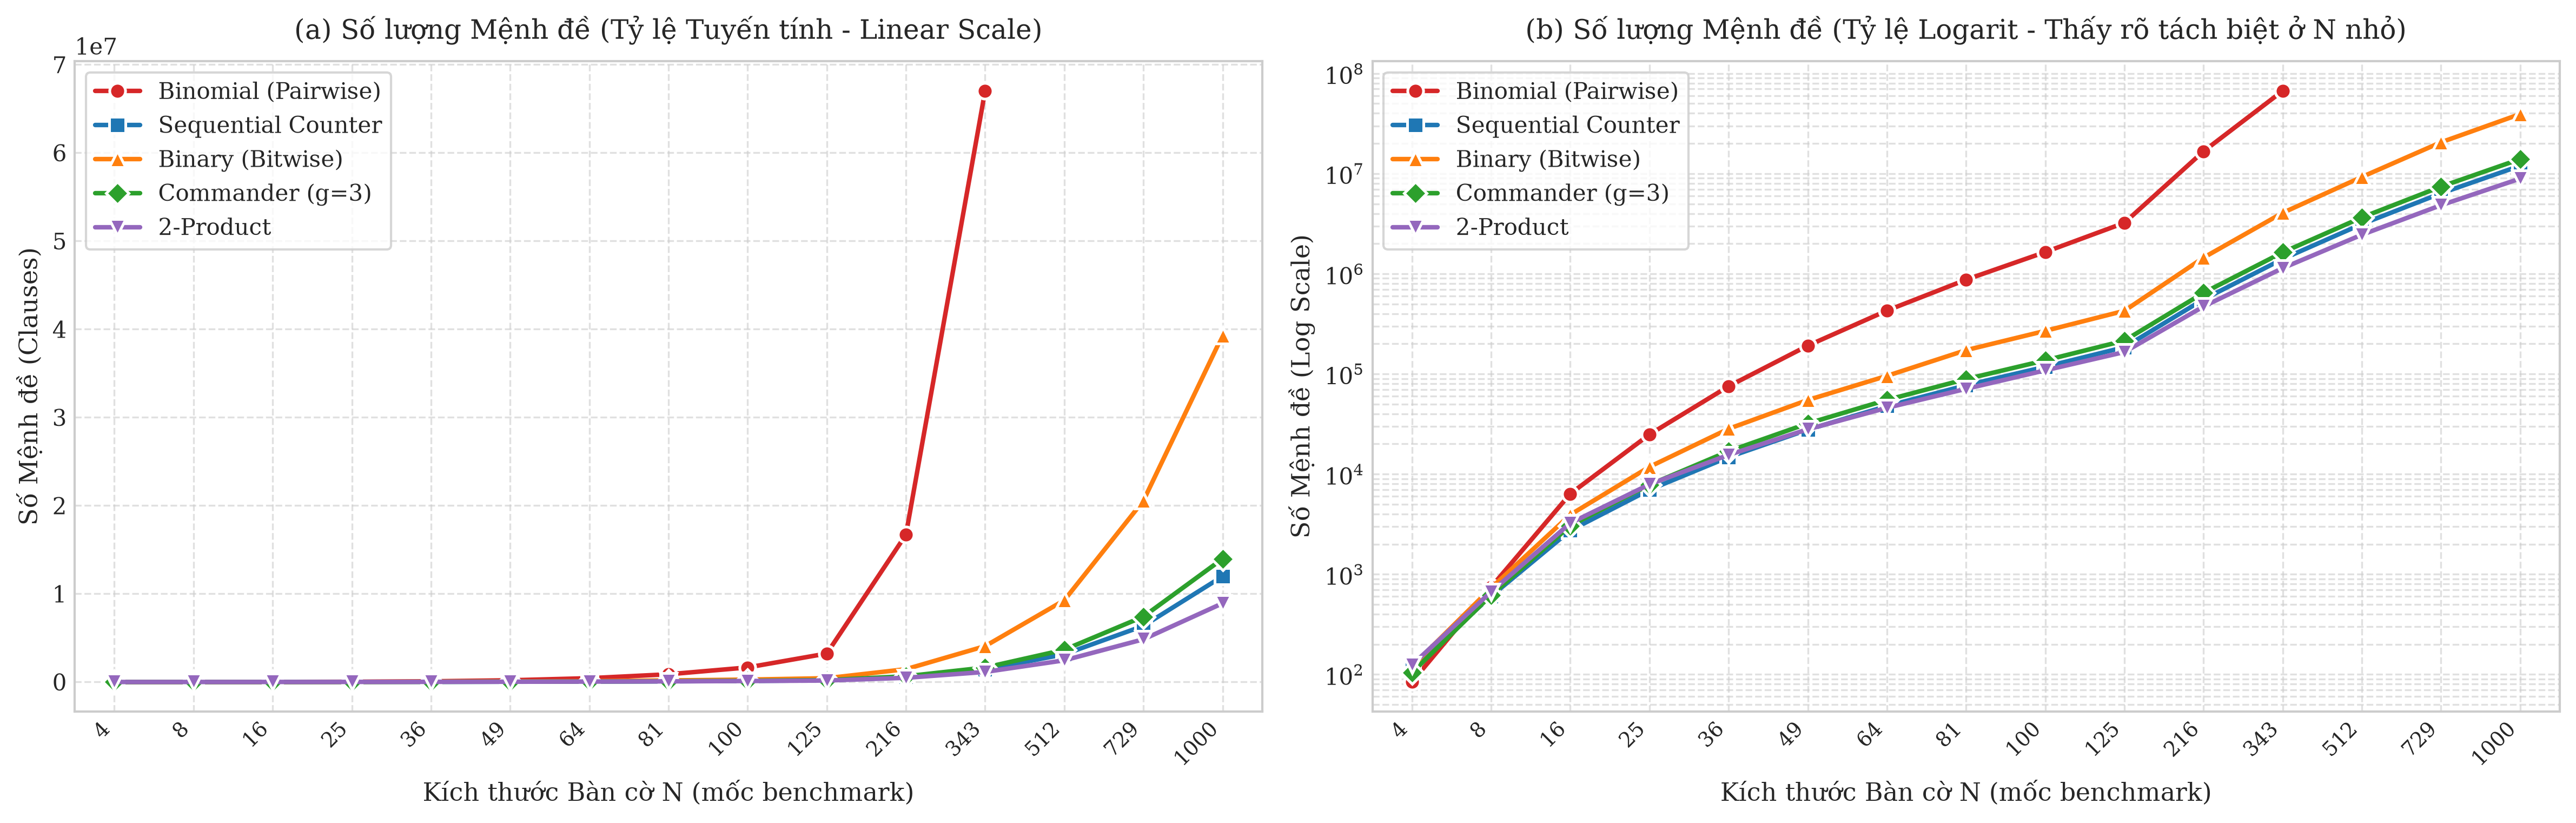
\includegraphics[width=0.92\linewidth]{results/figures/encoding_clauses.png}
    \caption{So sánh số lượng mệnh đề CNF sinh ra giữa 5 kỹ thuật mã hóa SAT qua 15 mốc kích thước ($N \in [4, 1000]$) trên thang đo tuyến tính (trái) và thang đo logarit (phải).}
    \label{fig:enc_clauses}
\end{figure*}

\begin{figure*}[htbp]
    \centering
    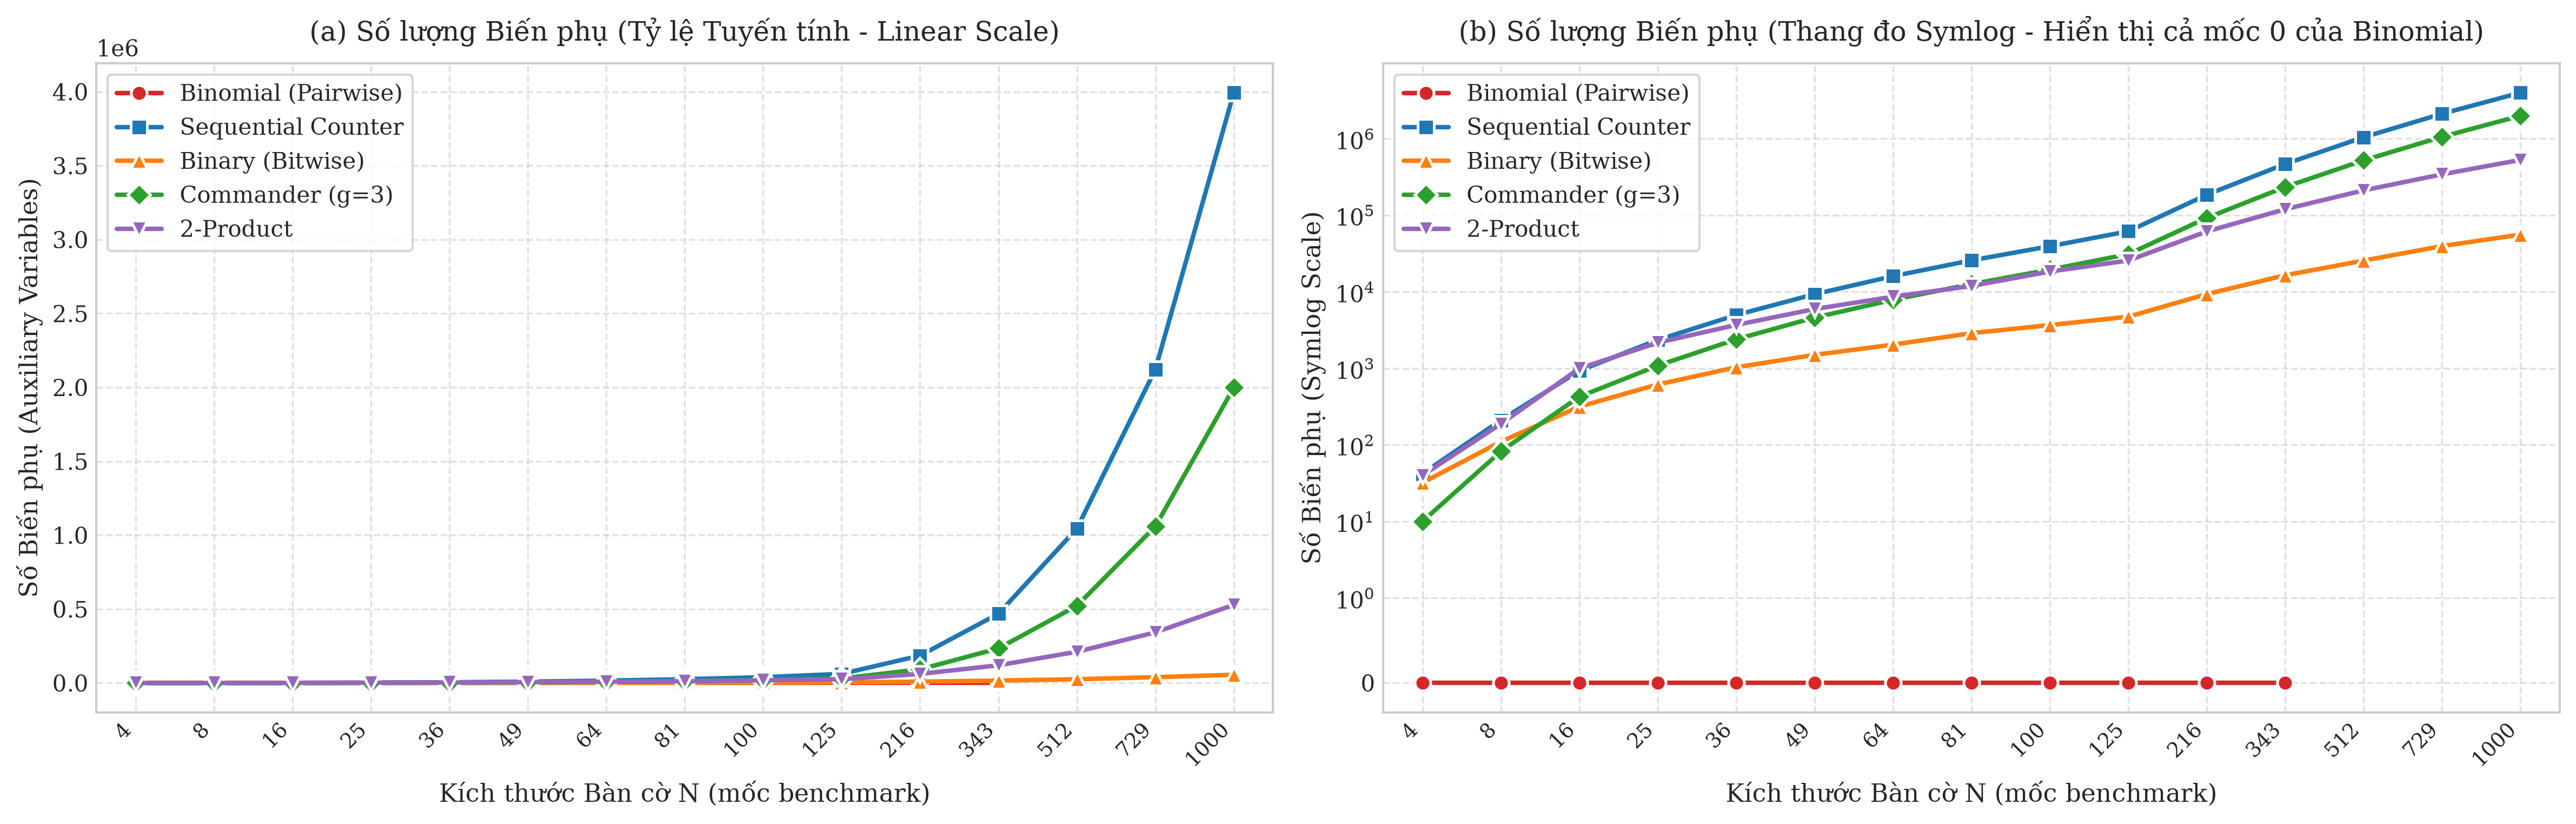
\includegraphics[width=0.92\linewidth]{results/figures/encoding_aux_vars.png}
    \caption{So sánh số lượng biến phụ trợ Boolean giữa 5 kỹ thuật mã hóa SAT qua 15 mốc kích thước ($N \in [4, 1000]$) trên thang đo tuyến tính (trái) và thang đo logarit đối xứng symlog (phải).}
    \label{fig:enc_aux_vars}
\end{figure*}

\begin{figure*}[htbp]
    \centering
    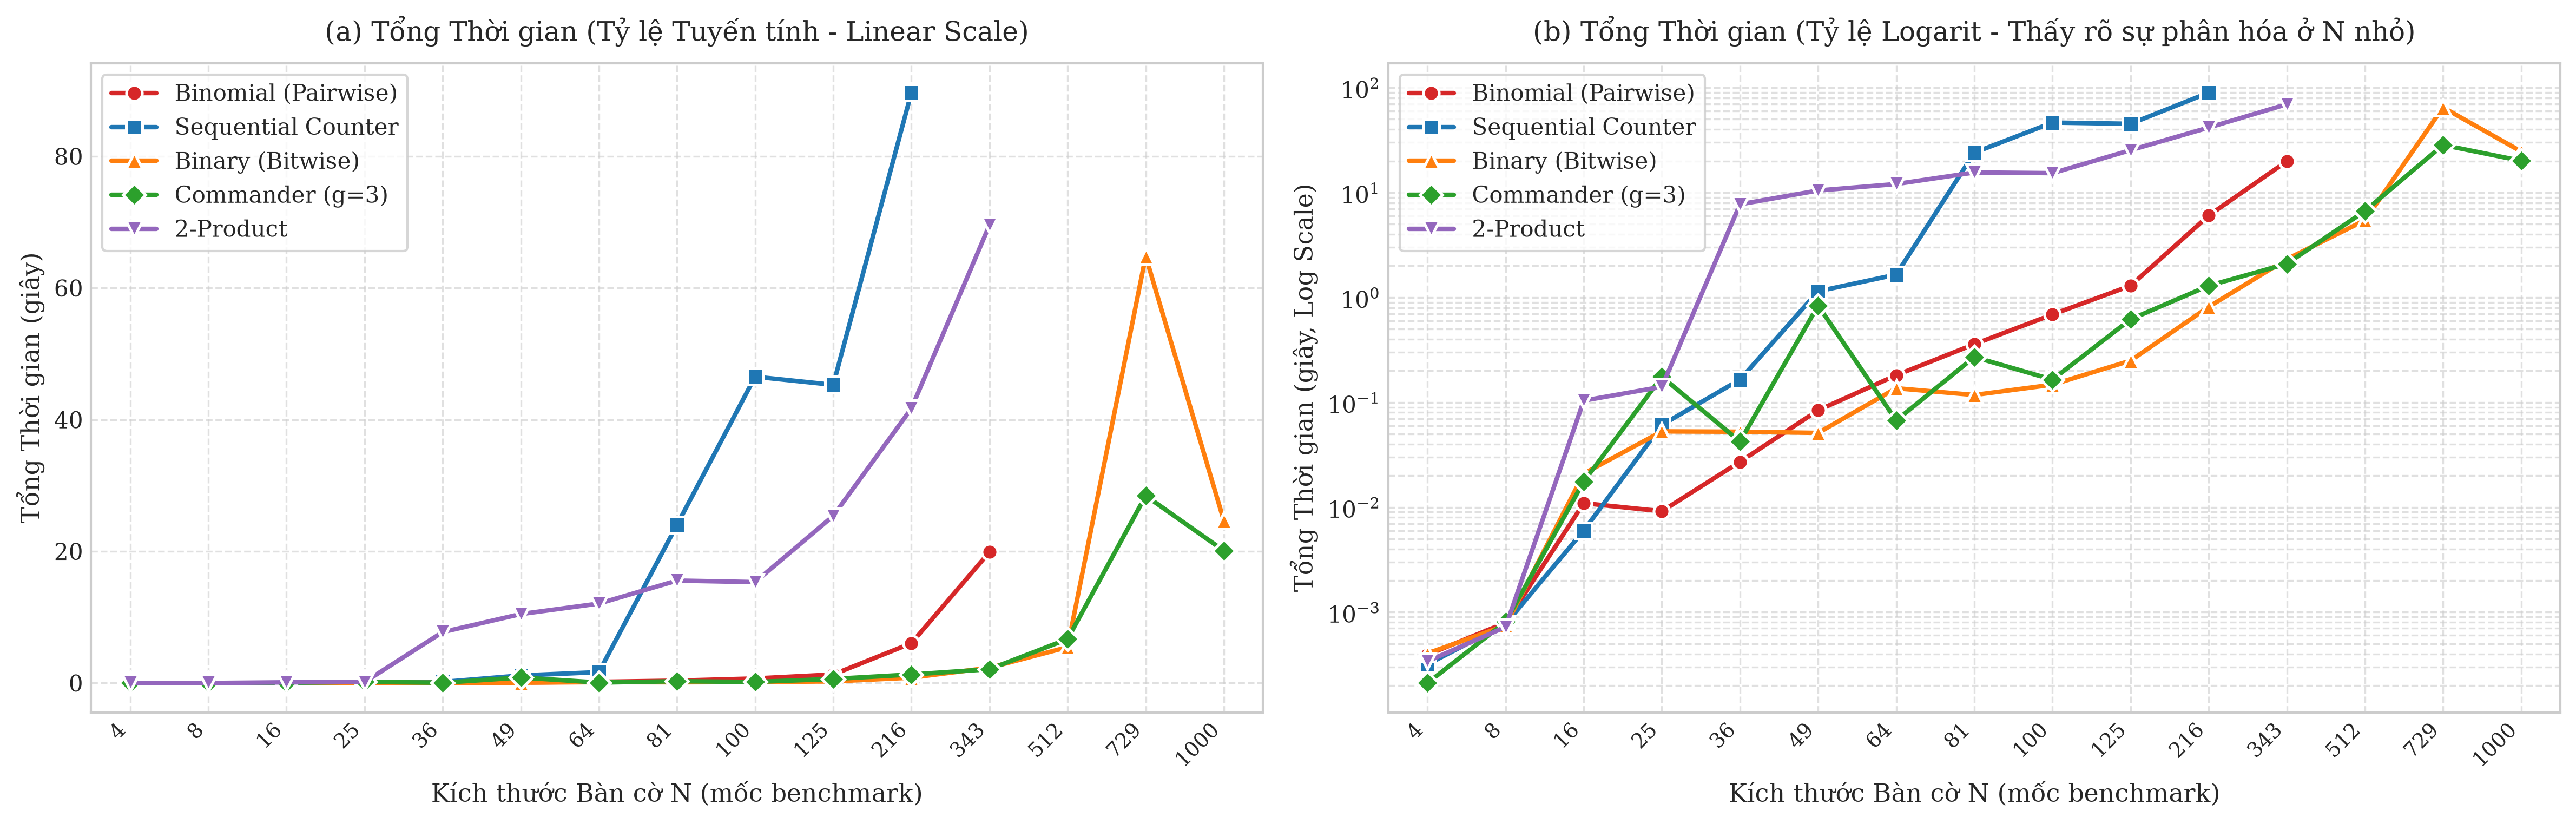
\includegraphics[width=0.92\linewidth]{results/figures/encoding_total_time.png}
    \caption{Tổng thời gian thực thi (thời gian sinh công thức + thời gian giải CDCL) của 5 kỹ thuật mã hóa SAT trên Glucose4 qua 15 mốc kích thước ($N \in [4, 1000]$) trên thang đo tuyến tính (trái) và thang đo logarit (phải).}
    \label{fig:enc_time}
\end{figure*}

\subsubsection{Phân tích Sâu về các Hiện tượng Thực nghiệm SAT Encodings}
Số liệu đo đạc thực nghiệm tại Bảng~\ref{tab:sat_encodings_results} cùng các đồ thị minh họa đã làm sáng tỏ năm hiện tượng bản chất chi phối hiệu năng của phương pháp SAT Solving:

\paragraph{1. Bức tường Bộ nhớ Binomial ($O(N^4)$)}
Mã hóa Binomial không sinh bất kỳ biến phụ nào và cho tốc độ giải nhanh nhất ở các kích thước nhỏ ($N \le 36$), ví dụ mốc $N=36$ chỉ mất $0{,}027$ giây. Tuy nhiên, tốc độ tăng trưởng số lượng mệnh đề bậc bốn khiến nó nhanh chóng trở thành thảm họa tài nguyên. Tại $N = 343$, nó sinh ra $67{,}021{,}514$ mệnh đề (tiêu tốn hơn $5{,}09$ giây chỉ để tạo công thức trong RAM), và dù Glucose4 vẫn kiên cường giải xong trong $14{,}80$ giây, thì việc tiến lên mốc $N = 512$ đã làm tràn hoàn toàn 16 GB RAM của máy trạm. Điều này khẳng định mã hóa cặp đôi truyền thống hoàn toàn bất khả thi cho các bài toán quy mô $N \ge 500$.

\paragraph{2. Nghịch lý Bộ đếm Tuần tự (Sequential Counter)}
Về mặt lý thuyết, Sequential Counter được đánh giá là mô hình mẫu mực vì vừa giữ số mệnh đề tuyến tính $O(m)$ vừa duy trì trọn vẹn Arc-Consistency (GAC) qua lan truyền đơn vị \cite{sinz2005towards}. Thế nhưng, thực nghiệm lại cho thấy đây là kỹ thuật nâng cao có hiệu năng kém nhất ở quy mô lớn, bị timeout ($> 120$s) ngay từ mốc $N = 343$.

Bản chất của nghịch lý này nằm ở sự xung đột giữa biến phụ và thuật toán phân nhánh CDCL. Tại $N = 1000$, Sequential Counter tạo ra tới $3{,}994{,}002$ biến phụ---gấp gần 4 lần số lượng biến quyết định ban đầu ($1{,}000{,}000$). Trong bộ giải CDCL, cơ chế VSIDS liên tục cộng điểm hoạt động cho các biến xuất hiện trong quá trình sinh mệnh đề xung đột. Vì các mệnh đề truyền thanh ghi $(\neg s_{i-1} \lor s_i)$ tham gia dày đặc vào các đồ thị hàm ý, bộ giải bị "đánh lừa" và liên tục chọn các biến thanh ghi phụ $s_i$ làm biến phân nhánh. Việc rẽ nhánh trên một biến tích lũy nội bộ có năng lực cắt tỉa không gian kém hơn rất nhiều so với việc rẽ nhánh trên một biến bàn cờ gốc $x_{i,j}$, khiến cây tìm kiếm bị phình to vô tận và dẫn tới hiện tượng nghẽn tìm kiếm (search thrashing).

\paragraph{3. Ưu thế Nén Biến Tuyệt vời của Mã hóa Nhị phân (Binary)}
Mã hóa Binary thể hiện sự vượt trội về khả năng kiểm soát số lượng biến phụ, chỉ cần $O(\log m)$ biến cho mỗi đường chéo hoặc hàng. Tại mốc cực đại $N = 1000$, mã hóa Binary chỉ cần thêm đúng $55{,}888$ biến phụ (chỉ chiếm $5{,}5\%$ so với 1 triệu biến gốc), trong khi Sequential Counter cần xấp xỉ 4 triệu biến và Commander cần 2 triệu biến. Dù số mệnh đề tăng ở mức $O(m \log m)$ ($39{,}300{,}904$ mệnh đề tại $N = 1000$), việc bảo toàn không gian biến giúp heuristic VSIDS tập trung trọn vẹn vào các biến quyết định thực sự. Kết quả là Binary giải thành công cả 15 mốc lên đến $N = 1000$ trong $24{,}66$ giây và đạt tốc độ dẫn đầu trong miền kích thước $N \in [49, 125]$.

\paragraph{4. Điểm Cân bằng Lý tưởng của Biến Chỉ huy (Commander Variable)}
Mã hóa Commander Variable ($g=3$) đạt được điểm dung hòa tối ưu nhất giữa số mệnh đề và số biến phụ. Nó duy trì lượng mệnh đề tuyến tính nghiêm ngặt ($13{,}968{,}946$ mệnh đề tại $N = 1000$, chỉ bằng $1/3$ so với Binary), đồng thời lượng biến phụ ($1{,}998{,}384$) được cấu trúc theo dạng cây phân cấp nhóm 3. Cấu trúc này hoạt động như một bộ phân rã bài toán tự nhiên: khi một biến chỉ huy bị gán False, lan truyền đơn vị lập tức loại bỏ đồng thời cả 3 ô cờ thành viên. Nhờ đó, Commander Variable là mã hóa SAT đạt tốc độ giải nhanh nhất ở mốc $N = 1000$ với tổng thời gian $20{,}10$ giây (thời gian giải thuần túy của Glucose4 chỉ là $16{,}42$ giây).

\paragraph{5. Đặc tính Thực nghiệm của Mã hóa 2-Product}
Mã hóa 2-Product duy trì số biến phụ ở mức $O(\sqrt{m})$ ($529{,}020$ biến tại $N = 1000$) và số mệnh đề tuyến tính ($8{,}922{,}032$ mệnh đề). Kỹ thuật này hoạt động hiệu quả đến mốc $N = 343$ ($69{,}55$ giây), nhưng chạm ngưỡng timeout tại $N \ge 512$. Nguyên nhân là cấu trúc phân rã lưới 2 chiều $p \times q$ tạo ra các mệnh đề phụ thuộc chéo; khi xảy ra xung đột, các mệnh đề học sinh ra có chỉ số LBD cao hơn, làm giảm tốc độ dọn dẹp bộ nhớ của Glucose4.

% -----------------------------------------------------------------------------
% MỤC: BENCHMARK ĐỐI ĐẦU ĐA MÔ HÌNH
% -----------------------------------------------------------------------------
\subsection{Benchmark Đa Mô hình Đối đầu: SAT vs. CP vs. MIP}
Để định vị năng lực cạnh tranh của phương pháp SAT Solving so với các trường phái tối ưu hóa chính xác khác, chúng tôi lựa chọn cấu hình SAT xuất sắc nhất---PySAT Glucose4 sử dụng mã hóa Commander Variable ($g=3$)---và tiến hành đối đầu trực diện với bốn bộ giải công nghiệp danh tiếng:
\begin{enumerate}
    \item \textbf{PySAT (Glucose4):} Bộ giải SAT CDCL với mã hóa Commander AMO.
    \item \textbf{Google OR-Tools (CP-SAT):} Engine lai CP/SAT sử dụng ràng buộc toàn cục $\text{AllDifferent}$.
    \item \textbf{IBM ILOG CPLEX (CP Optimizer):} Bộ giải Lập trình Ràng buộc chuyên biệt với thuật toán lọc Régin.
    \item \textbf{Gurobi Optimizer (MIP):} Bộ giải Quy hoạch Nguyên 0-1 thương mại hàng đầu thế giới.
    \item \textbf{IBM ILOG CPLEX (MIP):} Bộ giải Quy hoạch Nguyên 0-1 công nghiệp mạnh mẽ của IBM.
\end{enumerate}

Bảng~\ref{tab:cross_paradigm_results} cung cấp toàn bộ kết quả đối đầu qua 15 mốc kích thước, và Hình~\ref{fig:solver_time} biểu diễn đường cong thời gian thực thi trên thang đo tuyến tính và logarit.

\begin{table*}[t]
\centering
\caption{Bảng đối đầu thực nghiệm thời gian thực thi (giây) giữa ba trường phái giải chính xác: SAT (Glucose4 Commander), Constraint Programming (OR-Tools CP-SAT, CPLEX CP), và Mixed Integer Programming (Gurobi MIP, CPLEX MIP) qua 15 mốc kích thước ($N \in [4, 1000]$). Ký hiệu gạch ngang (-) biểu thị trường hợp quá thời gian (timeout $> 120.0$s).}
\label{tab:cross_paradigm_results}
\small
\setlength{\tabcolsep}{4.5pt}
\begin{tabular*}{\textwidth}{@{\extracolsep{\fill}} r | r r | r r | r r | r r | r r @{}}
\toprule
\multirow{2}{*}{$N$} 
 & \multicolumn{2}{c|}{\textbf{PySAT (Glucose4)}} 
 & \multicolumn{2}{c|}{\textbf{OR-Tools (CP-SAT)}} 
 & \multicolumn{2}{c|}{\textbf{IBM CPLEX (CP)}} 
 & \multicolumn{2}{c|}{\textbf{Gurobi (MIP)}} 
 & \multicolumn{2}{c}{\textbf{IBM CPLEX (MIP)}} \\
\cmidrule{2-3} \cmidrule{4-5} \cmidrule{6-7} \cmidrule{8-9} \cmidrule{10-11}
 & \textbf{T.gian (s)} & \textbf{T.thái} 
 & \textbf{T.gian (s)} & \textbf{T.thái} 
 & \textbf{T.gian (s)} & \textbf{T.thái} 
 & \textbf{T.gian (s)} & \textbf{T.thái} 
 & \textbf{T.gian (s)} & \textbf{T.thái} \\
\midrule
4 & \textbf{0.000354} & \texttt{SAT} & 0.006930 & \texttt{OPT} & 0.010402 & \texttt{FEAS} & 0.001436 & \texttt{OPT} & 0.027119 & \texttt{OPT} \\
8 & 0.000917 & \texttt{SAT} & 0.004844 & \texttt{OPT} & 0.008597 & \texttt{FEAS} & \textbf{0.000752} & \texttt{OPT} & 0.014829 & \texttt{OPT} \\
16 & 0.017303 & \texttt{SAT} & 0.011416 & \texttt{OPT} & 0.008362 & \texttt{FEAS} & \textbf{0.007822} & \texttt{OPT} & 0.016948 & \texttt{OPT} \\
25 & 0.172797 & \texttt{SAT} & 0.034547 & \texttt{OPT} & 0.014547 & \texttt{FEAS} & \textbf{0.002465} & \texttt{OPT} & 0.022689 & \texttt{OPT} \\
36 & 0.039431 & \texttt{SAT} & 0.039437 & \texttt{OPT} & \textbf{0.011243} & \texttt{FEAS} & 0.015984 & \texttt{OPT} & 0.036020 & \texttt{OPT} \\
49 & 0.815832 & \texttt{SAT} & 0.071425 & \texttt{OPT} & 0.010962 & \texttt{FEAS} & \textbf{0.008499} & \texttt{OPT} & 0.044594 & \texttt{OPT} \\
64 & 0.065774 & \texttt{SAT} & 0.147537 & \texttt{OPT} & 0.011249 & \texttt{FEAS} & \textbf{0.011147} & \texttt{OPT} & 0.071553 & \texttt{OPT} \\
81 & 0.280503 & \texttt{SAT} & 0.277318 & \texttt{OPT} & \textbf{0.013246} & \texttt{FEAS} & 0.017800 & \texttt{OPT} & 0.094604 & \texttt{OPT} \\
100 & 0.175485 & \texttt{SAT} & 0.445412 & \texttt{OPT} & \textbf{0.014226} & \texttt{FEAS} & 0.030660 & \texttt{OPT} & 0.126954 & \texttt{OPT} \\
125 & 0.665797 & \texttt{SAT} & 0.794817 & \texttt{OPT} & \textbf{0.018322} & \texttt{FEAS} & 0.043101 & \texttt{OPT} & 0.207947 & \texttt{OPT} \\
216 & 1.271689 & \texttt{SAT} & 9.934863 & \texttt{OPT} & \textbf{0.020885} & \texttt{FEAS} & 0.142422 & \texttt{OPT} & 0.660352 & \texttt{OPT} \\
343 & 2.139438 & \texttt{SAT} & 79.703568 & \texttt{OPT} & \textbf{0.038154} & \texttt{FEAS} & 0.360595 & \texttt{OPT} & 1.943252 & \texttt{OPT} \\
512 & 6.297810 & \texttt{SAT} & - & \texttt{TIMEOUT} & \textbf{0.072848} & \texttt{FEAS} & 0.838465 & \texttt{OPT} & 4.981404 & \texttt{OPT} \\
729 & 28.499749 & \texttt{SAT} & - & \texttt{TIMEOUT} & \textbf{0.125595} & \texttt{FEAS} & 24.102968 & \texttt{OPT} & 14.904806 & \texttt{OPT} \\
1000 & 18.918557 & \texttt{SAT} & - & \texttt{TIMEOUT} & \textbf{0.250158} & \texttt{FEAS} & - & \texttt{TIMEOUT} & 19.415871 & \texttt{OPT} \\
\bottomrule
\end{tabular*}
\end{table*}

\begin{figure*}[htbp]
    \centering
    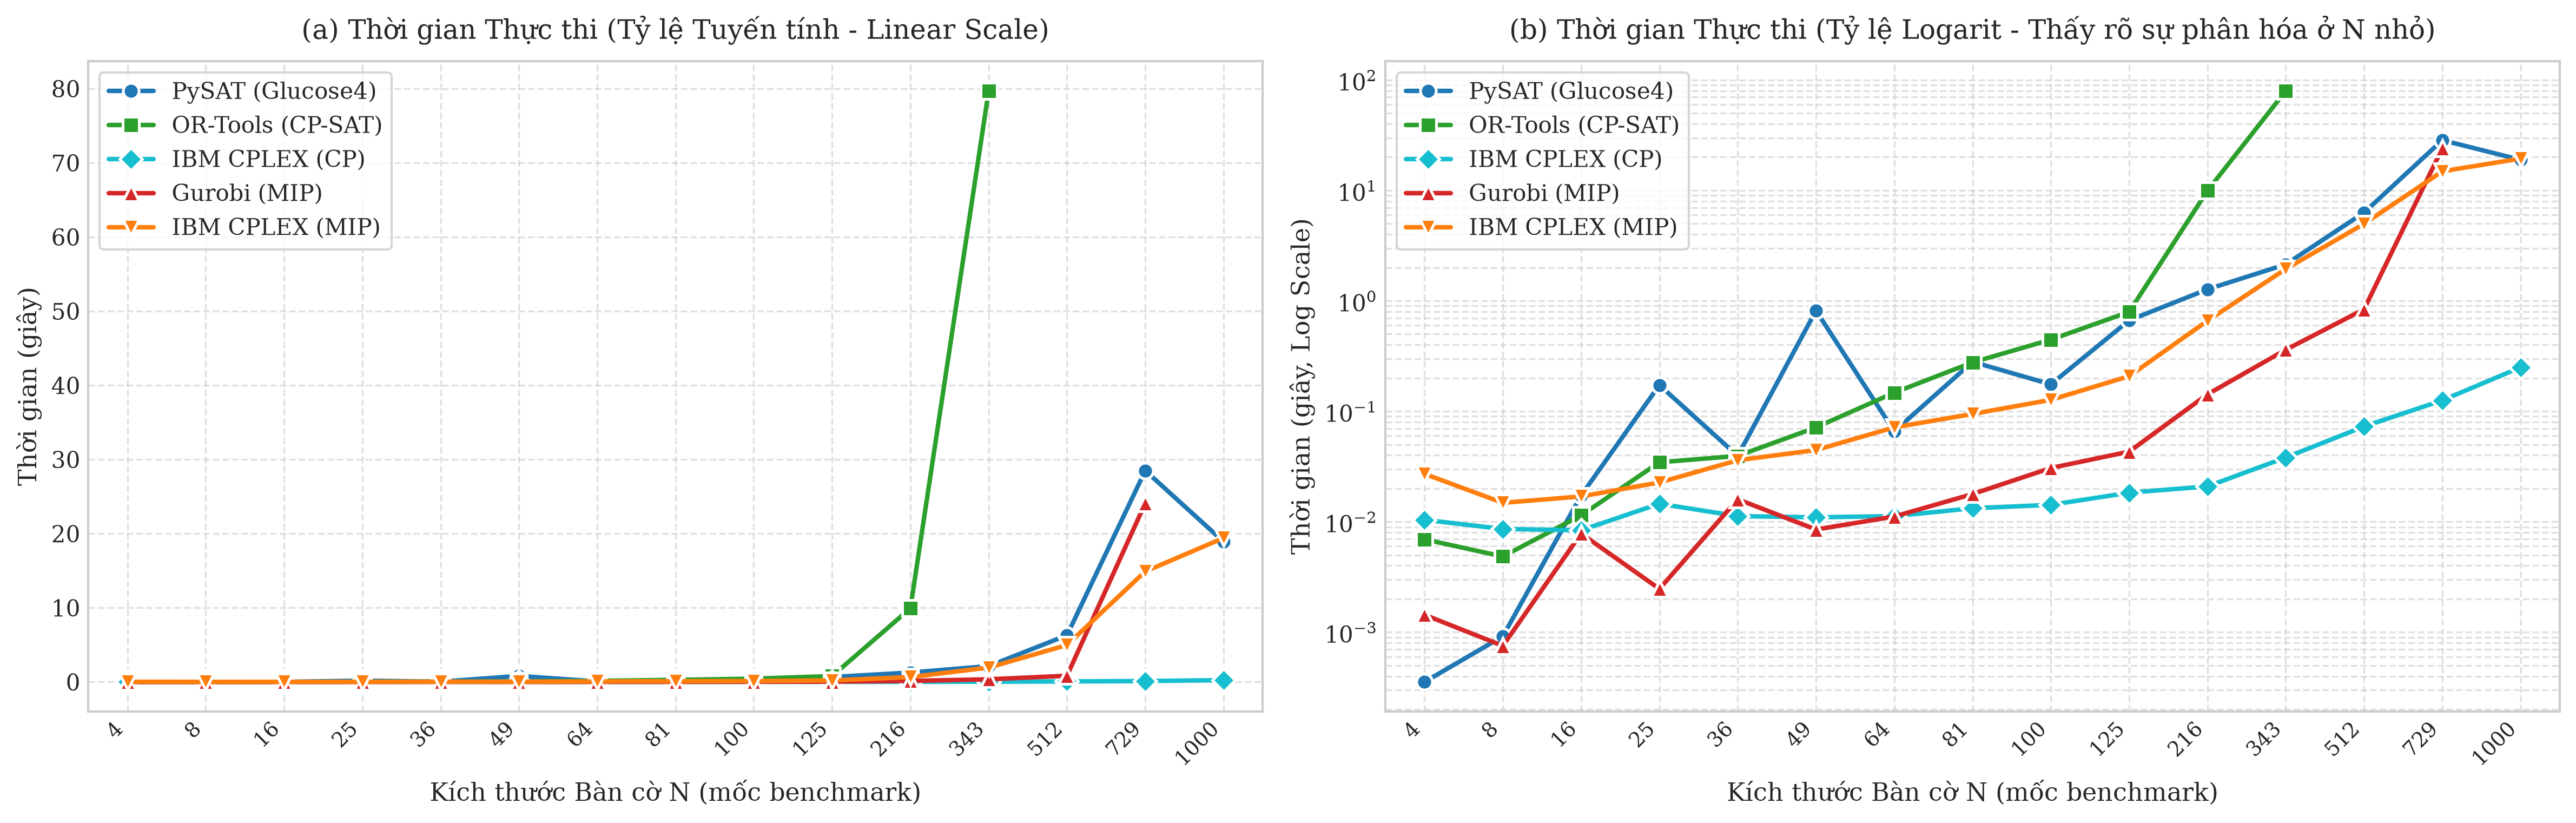
\includegraphics[width=0.92\linewidth]{results/figures/solver_total_time.png}
    \caption{So sánh thời gian thực thi đa mô hình (thang tuyến tính bên trái, thang logarit bên phải) giữa SAT (PySAT Glucose4 Commander), Lập trình ràng buộc CP (Google OR-Tools CP-SAT, IBM CPLEX CP), và Quy hoạch nguyên MIP (Gurobi MIP, IBM CPLEX MIP) qua 15 mốc kích thước ($N \in [4, 1000]$).}
    \label{fig:solver_time}
\end{figure*}

\subsubsection{Thảo luận Chi tiết về Hiệu năng Đa Mô hình}

\paragraph{1. IBM CPLEX CP Optimizer: Quán quân Tuyệt đối về Tốc độ}
Trong toàn bộ 15 mốc kích nghiệm, IBM CPLEX CP Optimizer thể hiện sự áp đảo toàn diện và tuyệt đối về tốc độ giải. Trong khi các bộ giải khác đều có thời gian chạy tăng dần theo hàm mũ hoặc đa thức bậc cao, CPLEX CP duy trì thời gian phản hồi ở mức mili-giây: giải $N=100$ chỉ trong $0{,}014$ giây, $N=512$ trong $0{,}073$ giây, và giải quyết bàn cờ cực đại $N=1000$ (1 triệu ô cờ) trong vỏn vẹn \textbf{$0{,}250$ giây}---nhanh hơn ít nhất $75$ lần so với bất kỳ bộ giải nào khác trong cuộc đua.

Thành tựu phi thường này minh chứng cho tính ưu việt của mô hình Lập trình Ràng buộc đối với các bài toán dạng hoán vị. Nhờ mô hình hóa bằng $N$ biến nguyên và 3 ràng buộc $\text{AllDifferent}$, CPLEX CP hoàn toàn tránh được việc phải khởi tạo 1 triệu biến nhị phân. Thuật toán cặp ghép cực đại của Régin thực hiện việc gọt tỉa miền giá trị thần tốc ngay tại nút gốc, loại bỏ hầu như toàn bộ các nhánh rẽ sai lầm trước khi quá trình phân nhánh bắt đầu.

\paragraph{2. Quy hoạch Tuyến tính Nguyên 0-1: Cuộc đua giữa Gurobi và CPLEX MIP}
Cả Gurobi và IBM CPLEX MIP đều chứng tỏ năng lực xử lý vượt trội trên các bài toán tối ưu hóa nhị phân chứa hàng trăm nghìn đến một triệu biến:
\begin{itemize}
    \item \textbf{Gurobi Optimizer:} Gurobi dẫn đầu về tốc độ ở miền kích thước vừa và lớn ($N \in [8, 49]$), giải mốc $N=49$ chỉ trong $0{,}008$ giây. Tại $N = 512$ ($262{,}144$ biến nhị phân), Gurobi tìm ra nghiệm nguyên chỉ sau $0{,}838$ giây, và giải xong $N = 729$ ($531{,}441$ biến) trong $24{,}10$ giây. Tuy nhiên, khi quy mô chạm mốc $1.000.000$ biến nhị phân ($N=1000$), bảng đơn vị và ma trận nới lỏng LP quá lớn khiến pha presolve và phân tích cơ sở đơn hình bị nghẽn, dẫn tới chạm ngưỡng timeout 120 giây.
    \item \textbf{IBM CPLEX MIP:} CPLEX MIP thể hiện độ bền bỉ và ổn định phi thường trên các mô hình siêu lớn. Solver này giải mốc $N = 512$ trong $4{,}98$ giây, $N = 729$ trong $14{,}90$ giây, và giải thành công bài toán 1 triệu biến nhị phân $N = 1000$ chỉ trong \textbf{$19{,}42$ giây}. Các thuật toán tinh chỉnh xung đột (conflict refiner) và lát cắt không-nửa (zero-half cuts) của CPLEX MIP đã chứng minh hiệu quả vượt trội trong việc triệt tiêu nghiệm phân số.
\end{itemize}

\paragraph{3. Google OR-Tools (CP-SAT)}
Google OR-Tools CP-SAT vận hành mượt mà ở các kích thước $N \le 125$ (dưới 1 giây) và giải thành công mốc $N = 343$ trong $79{,}70$ giây. Tuy nhiên, solver bắt đầu gặp timeout tại $N \ge 512$.

Nguyên nhân xuất phát từ kiến trúc lai của CP-SAT: khác với các engine CP thuần túy lọc trực tiếp trên miền giá trị đồ thị, CP-SAT giải quyết bài toán bằng cách phân rã (flattening) các ràng buộc toàn cục thành các mệnh đề Boolean và bất đẳng thức tuyến tính giả Boolean (pseudo-boolean) bên dưới một kiến trúc SAT lazy-clause \cite{perron2023ortools}. Khi $N$ tăng cao, quá trình sinh mệnh đề bên trong trở nên quá tải, dẫn tới tình trạng nghẽn tương tự như hiện tượng ta đã chứng kiến ở mã hóa Sequential Counter.

\paragraph{4. Năng lực Cạnh tranh Xuất sắc của SAT (Glucose4 Commander)}
Phát hiện thực nghiệm mang ý nghĩa khoa học lớn nhất chính là sự vươn lên mạnh mẽ của phương pháp SAT Solving. Khi được trang bị mã hóa Commander Variable, bộ giải mã nguồn mở PySAT Glucose4 đã giải quyết trọn vẹn cả 15 mốc kích thước, hoàn thành mốc $N = 1000$ trong \textbf{$18{,}92$ giây}.

Tại mốc $N = 1000$, Glucose4 đã đánh bại cả Google OR-Tools CP-SAT (bị timeout) lẫn Gurobi Optimizer (bị timeout), đồng thời đạt tốc độ nhỉnh hơn cả bộ giải thương mại IBM CPLEX MIP ($18{,}92$s so với $19{,}42$s). Kết quả này đập tan định kiến cho rằng SAT solver chỉ giải được các bài toán lý thuyết nhỏ, khẳng định rằng một bộ giải SAT CDCL hiện đại nếu được kết hợp cùng một kỹ thuật mã hóa AMO tối ưu hoàn toàn đủ sức so găng sòng phẳng với các bộ giải thương mại đắt đỏ hàng đầu thế giới.

\subsection{Ma trận Khuyến nghị Thực hành (Decision Matrix)}
Dựa trên các kết quả phân tích lý thuyết và thực nghiệm, chúng tôi tổng hợp ma trận khuyến nghị tại Bảng~\ref{tab:decision_matrix} nhằm định hướng cho các kỹ sư và nhà nghiên cứu trong việc lựa chọn trường phái giải và kỹ thuật mã hóa phù hợp nhất cho các bài toán tổ hợp thực tế.

\begin{table}[htbp]
\centering
\caption{Ma trận khuyến nghị lựa chọn trường phái giải và kỹ thuật mã hóa dựa trên quy mô và đặc trưng bài toán.}
\label{tab:decision_matrix}
\small
\begin{tabular*}{\tblwidth}{@{} LLL @{}}
\toprule
\textbf{Quy mô / Đặc trưng Bài toán} & \textbf{Trường phái / Bộ giải Khuyến nghị} & \textbf{Lý do và Điểm mấu chốt} \\
\midrule
Quy mô nhỏ ($N \le 36$) & Binomial SAT hoặc Gurobi MIP & Không tốn biến phụ; suy diễn trực tiếp tức thì. \\
Quy mô vừa ($36 < N \le 125$) & Binary SAT hoặc Gurobi MIP & Tiết kiệm biến phụ tối đa; presolve tuyến tính mạnh. \\
Quy mô lớn ($125 < N \le 500$) & Commander SAT hoặc CPLEX MIP & Cân bằng mệnh đề/biến phụ; nhánh cận ổn định. \\
Quy mô cực đại ($N \ge 500$) & \textbf{IBM CPLEX CP Optimizer} & Chỉ $N$ biến nguyên; lọc miền giá trị đa thức siêu tốc. \\
Mô hình logic thuần túy / Mã nguồn mở & \textbf{PySAT (Commander / Binary)} & Quy mô triệu biến; không phụ thuộc bản quyền thương mại. \\
\bottomrule
\end{tabular*}
\end{table}

% -----------------------------------------------------------------------------
% MỤC 5: KẾT LUẬN VÀ HƯỚNG PHÁT TRIỂN
% -----------------------------------------------------------------------------
\section{Kết luận và Hướng Phát triển}
\label{sec:conclusion}

Bài báo đã hoàn thành một nghiên cứu thực nghiệm và lý thuyết chuyên sâu về các kỹ thuật mã hóa SAT và so sánh đa mô hình giải chính xác cho bài toán $N$-Queens. Thông qua hệ thống benchmark chuẩn hóa trên 15 mốc kích thước từ $N = 4$ đến $N = 1000$ (tương ứng $1.000.000$ biến nhị phân), chúng tôi đã đánh giá toàn diện năm phương pháp mã hóa At-Most-One (AMO) trên Glucose4 và đối đầu trực diện với bốn bộ giải công nghiệp hàng đầu thuộc trường phái CP và MIP.

Các kết luận khoa học cốt lõi bao gồm:
\begin{enumerate}
    \item Mã hóa Binomial dù rất nhanh ở kích thước nhỏ nhưng chạm bức tường bộ nhớ vật lý tại $N \ge 512$ do số mệnh đề tăng trưởng bậc bốn $O(N^4)$.
    \item Việc bảo toàn tính nhất quán cung tổng quát (GAC) trên lý thuyết không đồng nghĩa với hiệu năng giải nhanh: Sequential Counter thất bại tại $N \ge 343$ do lượng biến phụ khổng lồ làm loãng heuristic rẽ nhánh CDCL.
    \item Mã hóa Binary ($O(\log m)$ biến phụ) và mã hóa Commander Variable ($g=3$) là hai kỹ thuật mã hóa xuất sắc nhất, cho phép Glucose4 giải quyết thành công mốc $N = 1000$ trong chưa đầy 19 giây.
    \item Lập trình Ràng buộc (CP) với thuật toán lọc cặp ghép cực đại của Régin trên ràng buộc toàn cục $\text{AllDifferent}$ là trường phái vô địch tuyệt đối về tốc độ giải bài toán $N$-Queens, với thời gian giải $0{,}250$ giây cho $N = 1000$ của IBM CPLEX CP.
    \item Phương pháp SAT Solving (với mã hóa Commander) chứng minh năng lực cạnh tranh vượt trội, đánh bại cả Gurobi lẫn Google OR-Tools CP-SAT tại $N = 1000$, mở ra tiềm năng ứng dụng to lớn của các bộ giải SAT mã nguồn mở cho các bài toán thỏa mãn ràng buộc quy mô công nghiệp.
\end{enumerate}

\subsection{Hướng Nghiên cứu Tiếp theo}
Từ các kết quả đạt được, một số hướng nghiên cứu giàu triển vọng bao gồm:
\begin{itemize}
    \item \textbf{Phá vỡ Tính Đối xứng (Symmetry Breaking Constraints - SBC):} Bàn cờ sở hữu tính đối xứng xoay và phản xạ thuộc nhóm nhị diện $D_4$ cấp 8. Việc tích hợp các mệnh đề phá vỡ đối xứng (như Lex-Leader) hứa hẹn sẽ thu hẹp không gian tìm kiếm hơn nữa cho các bộ giải SAT và MIP \cite{crawford1996symmetry}.
    \item \textbf{Khảo sát Bộ giải SAT Song song:} Đánh giá trên các bộ giải SAT song song và portfolio solver hàng đầu thế giới hiện nay như Kissat, CaDiCaL, và CryptoMiniSAT \cite{biere2009handbook}.
    \item \textbf{Mở rộng sang các Biến thể Tối ưu hóa:} Áp dụng các kỹ thuật mã hóa này cho các bài toán mở rộng như Xếp quân hậu không tấn công cực đại (Maximum Non-Attacking Queens) hoặc bài toán Thống trị quân hậu (Queens Domination) thông qua giải thuật MaxSAT và SAT tăng dần (Incremental SAT).
\end{itemize}

% -----------------------------------------------------------------------------
% CREDIT AUTHORSHIP CONTRIBUTION STATEMENT
% -----------------------------------------------------------------------------
\section*{Đóng góp của tác giả (CRediT authorship contribution statement)}
\textbf{Trần Nhật Hưng:} Khởi xướng ý tưởng (Conceptualization), Phương pháp luận (Methodology), Phát triển phần mềm (Software), Phân tích hình thức (Formal analysis), Điều tra thực nghiệm (Investigation), Quản lý dữ liệu (Data curation), Trực quan hóa (Visualization), Viết bản thảo gốc (Writing -- original draft), Soát xét và chỉnh sửa (Writing -- review \& editing).

% -----------------------------------------------------------------------------
% DECLARATION OF COMPETING INTEREST
% -----------------------------------------------------------------------------
\section*{Tuyên bố xung đột lợi ích (Declaration of competing interest)}
Tác giả khẳng định rằng không có bất kỳ xung đột lợi ích tài chính hoặc mối quan hệ cá nhân nào có thể ảnh hưởng đến các kết quả nghiên cứu được công bố trong bài báo này.

% -----------------------------------------------------------------------------
% DATA AVAILABILITY
% -----------------------------------------------------------------------------
\section*{Tính sẵn sàng của dữ liệu và mã nguồn (Data availability)}
Toàn bộ mã nguồn triển khai các solver, bộ công cụ tự động hóa benchmark, dữ liệu thực nghiệm thô dạng CSV và các notebook phân tích trực quan hóa được công khai minh bạch tại kho lưu trữ GitHub của đề tài:
\begin{center}
\url{https://github.com/NhHung07/N_Queens.git}
\end{center}

% -----------------------------------------------------------------------------
% ACKNOWLEDGEMENTS
% -----------------------------------------------------------------------------
\section*{Lời cảm ơn (Acknowledgements)}
Tác giả xin bày tỏ lòng biết ơn chân thành và sâu sắc nhất tới TS. Tô Văn Khánh (Khoa Công nghệ Thông tin, Trường Đại học Công nghệ, Đại học Quốc gia Hà Nội) vì sự hướng dẫn tận tâm, các bài giảng nền tảng trong học phần Các vấn đề hiện đại trong Khoa học Máy tính, cùng những định hướng học thuật quý báu về các kỹ thuật mã hóa SAT và tối ưu hóa tổ hợp.

% -----------------------------------------------------------------------------
% TÀI LIỆU THAM KHẢO
% -----------------------------------------------------------------------------
\begin{thebibliography}{99}

\bibitem{bezzel1848}
M.~Bezzel, Schachfreund, Berliner Schachzeitung 3 (1848) 363.

\bibitem{nauck1850}
F.~Nauck, Briefwechsel mit allen f{\"u}r alle, Illustrirte Zeitung 15 (377) (1850) 182.

\bibitem{bell2009survey}
J.~Bell, B.~Stevens, A survey of known results and research areas for n-queens, Discrete Mathematics 309~(1) (2009) 1--31.
\newblock \href {https://doi.org/10.1016/j.disc.2007.12.043} {\path{doi:10.1016/j.disc.2007.12.043}}.

\bibitem{sosic1994polynomial}
R.~Sosic, J.~Gu, Efficient local search with conflict minimization: A polynomial-time algorithm for the n-queens problem, IEEE Transactions on Knowledge and Data Engineering 6~(5) (1994) 661--668.

\bibitem{erbas1992queens}
C.~Erbas, M.~M. Tanik, Generating solutions to the n-queens problem using 2-circulant matrices, Computers \& Mathematics with Applications 24~(11) (1992) 89--97.

\bibitem{golomb1965backtrack}
S.~W. Golomb, L.~D. Baumert, Backtrack programming, Journal of the ACM 12~(4) (1965) 516--524.

\bibitem{bitner1975backtrack}
J.~R. Bitner, E.~M. Reingold, Backtrack programming techniques, Communications of the ACM 18~(11) (1975) 651--656.

\bibitem{biere2009handbook}
A.~Biere, M.~Heule, H.~van Maaren, T.~Walsh (Eds.), Handbook of Satisfiability, Vol. 185 of Frontiers in Artificial Intelligence and Applications, IOS Press, Amsterdam, 2009.

\bibitem{audemard2009predicting}
G.~Audemard, L.~Simon, Predicting learnt clauses quality in modern SAT solvers, in: Proceedings of the 21st International Joint Conference on Artificial Intelligence (IJCAI'09), Morgan Kaufmann Publishers, 2009, pp. 399--404.

\bibitem{moskewicz2001chaff}
M.~W. Moskewicz, C.~F. Madigan, Y.~Zhao, L.~Zhang, S.~Malik, Chaff: Accelerating engineering SAT runtimes, in: Proceedings of the 38th Design Automation Conference (DAC'01), ACM, 2001, pp. 530--535.

\bibitem{regin1994filtering}
J.-C. R{\'e}gin, A filtering algorithm for constraints of difference in CSPs, in: Proceedings of the 12th National Conference on Artificial Intelligence (AAAI'94), AAAI Press, 1994, pp. 362--367.

\bibitem{rossi2006handbook}
F.~Rossi, P.~van Beek, T.~Walsh (Eds.), Handbook of Constraint Programming, Elsevier, Amsterdam, 2006.

\bibitem{wolsey1999integer}
L.~A. Wolsey, Integer Programming, John Wiley \& Sons, New York, 1999.

\bibitem{nemhauser1988integer}
G.~L. Nemhauser, L.~A. Wolsey, Integer and Combinatorial Optimization, John Wiley \& Sons, New York, 1988.

\bibitem{sinz2005towards}
C.~Sinz, Towards an optimal CNF encoding of boolean cardinality constraints, in: P.~van Beek (Ed.), Principles and Practice of Constraint Programming (CP 2005), Vol. 3709 of Lecture Notes in Computer Science, Springer, Berlin, Heidelberg, 2005, pp. 827--831.
\newblock \href {https://doi.org/10.1007/11564751_73} {\path{doi:10.1007/11564751_73}}.

\bibitem{klieber2007commander}
W.~Klieber, G.~Kwon, Efficient CNF encoding for selecting at most one item from a group, in: Proceedings of the International Workshop on Constraints in Formal Verification (CFV'07), 2007, pp. 1--9.

\bibitem{chen2010new}
J.~Chen, A new SAT encoding of the at-most-one constraint, in: Proceedings of the 10th International Conference on Formal Methods in Computer-Aided Design (FMCAD'10), 2010, pp. 268--275.

\bibitem{frisch2005atmost}
A.~M. Frisch, P.~A. Giannaros, SAT encodings of the at-most-k constraint, in: Proceedings of the 3rd International Workshop on Modelling and Reformulating Constraint Satisfaction Problems, 2005, pp. 45--56.

\bibitem{gent2002arc}
I.~P. Gent, Arc consistency in SAT, in: F.~van Harmelen (Ed.), Proceedings of the 15th European Conference on Artificial Intelligence (ECAI'02), IOS Press, 2002, pp. 121--125.

\bibitem{ignatiev2018pysat}
A.~Ignatiev, A.~Morgado, J.~Marques-Silva, PySAT: A Python library for prototyping with SAT oracles, in: J.~Beyer, M.~Henzinger (Eds.), Theory and Applications of Satisfiability Testing (SAT 2018), Vol. 10929 of Lecture Notes in Computer Science, Springer, Cham, 2018, pp. 428--437.
\newblock \href {https://doi.org/10.1007/978-3-319-94144-8_26} {\path{doi:10.1007/978-3-319-94144-8_26}}.

\bibitem{perron2023ortools}
L.~Perron, F.~Didier, CP-SAT solver, Google OR-Tools, \url{https://developers.google.com/optimization/cp/cp_solver} (2023).

\bibitem{bixby2002solving}
R.~E. Bixby, Solving real-world linear programs: A decade and more of progress, Operations Research 50~(1) (2002) 3--15.

\bibitem{achterberg2013gurobi}
T.~Achterberg, R.~Wunderling, Mixed integer programming: Analyzing 12 years of progress, in: Facets of Combinatorial Optimization, Springer, Berlin, Heidelberg, 2013, pp. 449--481.

\bibitem{crawford1996symmetry}
J.~Crawford, M.~Ginsberg, E.~Luks, A.~Roy, Symmetry-breaking predicates for search problems, in: Proceedings of the 5th International Conference on Principles of Knowledge Representation and Reasoning (KR'96), Morgan Kaufmann, 1996, pp. 148--159.

\bibitem{hung2026github}
T.~N. Hưng, Nghiên cứu thực nghiệm SAT encodings và so sánh đa mô hình cho bài toán N-Queens, Kho lưu trữ GitHub, \url{https://github.com/NhHung07/N_Queens.git} (2026).

\end{thebibliography}

\end{document}
